%--------------------------------------------------
% CHAPTER: Finite group gauge theories
%--------------------------------------------------
\chapter{Finite Group Gauge Theories}
\label{chap:finite_group_gauge_theories}

% In this chapter we present the work \cite{pradhan_unpublished}.
% We first start by reviewing the Kogut-Susskind Hamiltonian formulation of \acp{lgt}, which works for compact Lie groups.
% Next we will see how to transition from compact Lie groups to finite groups.
% With, we will present the main results of \cite{pradhan_unpublished}, which is the construction of the Hamiltonian and the physical Hilbert space.

In this chapter we present the work \cite{pradhan_unpublished}, where a class of finite-group gauge theories in the Hamiltonian formulation, which mimic some aspects of Lie group Yang-Mills theories on the lattice.
The Hamiltonian is based on the construction of a natural Laplacian operator on the finite group, and is valid for any Abelian or non-Abelian finite group.
As a special case, this includes both the finite-group Hamiltonian obtained via the transfer-matrix formulation from the finite-group Wilson action, but also a wider class of non-Lorentz invariant theories which could be relevant for condensed matter systems.
The characterization of the Hamiltonian using the finite-group Laplacian may be used to obtain non-trivial physical information about the theory.
Irrespective of the choice of Hamiltonian, we show that spin-network states are particularly suitable to give a description of the physical, gauge-invariant Hilbert space for pure gauge theories, and, based on this, we derive a simple formula to compute the dimension of the physical Hilbert space.
Finally, we illustrate the use of the gauge-invariant basis by constructing the Hamiltonian for a gauge theory based on the dihedral group and compute some quantities of interest via exact diagonalization.


% SECTION: Kogut-Susskind Hamiltonian
% %----------------------------------------
% SECTION: Kogut-Susskind Hamiltonian
%----------------------------------------
\section{Kogut-Susskind Hamiltonian formulation}
\label{sec:kogut_susskind_hamiltonian_formulation}

The classical formulation of Hamiltonian LTG is due to Kogut and Susskind, in \citneeded.
It can be regarded as the Hamiltonian corresponding to the Wilson action \todo{inserire eqref}.
The former can be obtained from the latter by the transfer matrix technique\citneeded, where two different lattice spacing are assigned to time and spatial dimensions and then the continuum limit for the time direction is taken.
Another derivation can be done by means of Legendre transform, but in this text we will adopt a more modern approach, based on \todo{citare Milsted, Osborne 2018}.

As one can expect, the Kogut-Susskind Hamiltonian $\HamilKS$ is made of two terms, the electric part and the magnetic part:
\begin{equation}
    \HamilKS = H_E + H_B.
\end{equation}
These will be constructed separately and for a simple reason.
The magnetic term involves only the spatial component of the field strength tensor, i.e., $\bm{B}^{2} \sim F^{ij}F_{ij}$, while the electric term involves also the temporal components, i.e., $\bm{E}^2 \sim F^{0i} F_{0i}$.
Given that in the Hamiltonian formalism time is continuous while space is discrete, the two terms cannot be treated on the same footing.
This differs from the Wilson action approach, where the magnetic and electric are treated equally because it has to be Lorentz-invariant.

% Starting from the magnetic term, this can be taken to be the same as the single-plaquette term in the Wilson action \eqref{eq:wilson_action}, but we have to limit ourselves to purely spatial plaquettes.
% In fact, the magnetic energy is $\bm{B}^2 = \frac{1}{2} F^{ij} F_{ij}$, which is just the spatial part of $F^{\mu \nu} F_{\mu \nu}$ of the continuum action.
% Given that the spatial directions are kept discrete, we do not need to make any modification.
% The same cannot be said for the electric energy, which is $\bm{E}^2 = F_{0 i} F^{0 i}$.
% With continuous time we cannot construct plaquettes that extends in the time direction.

Another point of divergence with the path-integral approach is that now both the electric field and magnetic term are operators, not simple variables.
In order to have well-defined, or defined at all, operators we have to define the appropriate Hilbert space on which these operators act.


% SUBSECTION: Single link Hilbert space and operators
\subsection{Single link Hilbert space and operators}
\label{sub:single_link_hilbert_space_and_operators}

We start by considering a single link $\link$ and define the gauge \ac{dof}.
In  the construction in Sec.~\ref{sub:gauge_fields_on_a_lattice}, given a gauge group $G$ we have associated an element $g \in G$ to the link $\link$.
Hence, the configuration space for each link $\link$ is exactly $G$.
When quantizing, the configuration space $G$ is elevated to a Hilbert space $\HilbertSpace^G$ which is spanned by the elements $g \in G$:
\begin{equation}
    \HilbertSpace^G \equiv \text{span}\{\ket{g} : g \in G\},
    \label{eq:single_link_Hilbert_space}
\end{equation}
where the set $\{\ket{g}\}$ is an orthonormal basis.
Therefore, an element $\ket{\psi}$ of $\HilbertSpace^G$ can be written as
\begin{equation}
    \ket{\psi} = \int \dd g \; \psi(g) \ket{g},
\end{equation}
where $\int \dd g$ is a proper measure in the case of continuous groups (usually the Haar measure) or a simple sum in case of finite groups.
In the former case $\HilbertSpace^G$ is equivalent to the space $L^2(G)$ of square-integrable functions of $G$, i.e., each element $\ket{\psi}$ can be identified with the functions $\psi(g)$.
While in the latter case, the space $\HilbertSpace^G$ is equivalent to the so-called group algebra $\C[G]$.
The total Hilbert space of the model is simply given by the tensor product
\begin{equation}
    \HilbertSpace_{\text{tot}} = \bigotimes_{\link} \HilbertSpace^G_{\link}
\end{equation}


Focusing now on the case of continuous groups like $\SU(N)$,
given a single link Hilbert space $\HilbertSpace^G_{\link}$, the first set of operators we can define on it are the \emph{position observables} $\transport_{mn}$, via
\begin{equation}
    \transport_{mn} \ket{g} = U(g)_{mn} \ket{g},
\end{equation}
where $U(g)_{mn}$ is the matrix element $(m, n)$ of $U(g)$, the image of $g$ in the fundamental representation $U$ of $G$.
One can then define a matrix of operators $\transport$, whose elements are precisely the operators $\transport_{mn}$.
Note that $\transport$ is unitary as long as the chosen representation is unitary, but this not guarantee that each operator $\transport_{mn}$ is unitary.
Indeed, it can be shown that $(\transport_{mn})^{\dagger} = (\transport^{\dagger})_{mn}$.

A second set of operators can be defined on $\HilbertSpace^G$, which makes use of the group structure of $G$.
For each element $h \in G$, we define $L_h$ and $R_h$ such that for any $\ket{g} \in G$
\begin{equation}
    L_h \ket{g} = \ket{hg}
    \qand
    R_h \ket{g} = \ket*{gh^{-1}},
\end{equation}
which are the \emph{left} and \emph{right} multiplication operators, respectively.
If the basis $\{\ket{g}\}$ is considered as the ``position basis'' then the operators $L_h$ and $R_h$ can be regarded as ``translation operators''.
The left multiplications commutes with the rights one and both $L_h$ and $R_h$ respects the group structure of $G$, i.e.,
\begin{equation}
    L_g L_h = L_{gh}
    \qand
    R_g R_h = R_{gh},
\end{equation}
indeed the maps $\hat{L}: h \mapsto L_h$ and $\hat{R}: h \mapsto R_h$ are basically \emph{regular representations} of the group $G$.
It can also be shown that $L_h$ and $R_h$ are unitary operators and satisfy
\begin{equation}
    (L_h)^{\dagger} = (L_h)^{-1} = L_{h^{-1}}
    \qand
    (R_h)^{\dagger} = (R_h)^{-1} = R_{h^{-1}}.
\end{equation}


\subsection{Magnetic Hamiltonian}
\label{sub:magnetic_hamiltonian}

As already mentioned, it is relatively easy to obtain the magnetic term if we already know the Wilson approach but it order to make the presentation clear we repeat the step for major clarity.

Fixing the lattice orientation, on a link $\link$ we define
\begin{equation}
    \transport_{mn}(\link) =
    \begin{cases}
        \transport_{mn} & \text{if $\link$ traversed in the positive direction}, \\
        \transport_{mn}^{\dagger} & \text{if $\link$ traversed in the negative direction}.
    \end{cases}
\end{equation}
Then, let $\gamma$ be a oriented path, which we write as $\gamma = \ev*{\link_1 \link_2 \dots \link_q}$.
Next, on $\gamma$ we can define the \emph{Wilson line} $W_{\gamma}$ whose matrix elements are
\begin{equation}
    (W_{\gamma})_{mn} =
    \sum_{m_1 \dots m_{q-1}}
        \transport_{m m_1} (\link_1)
        \transport_{m_1 m_2} (\link_2)
        \cdots
        \transport_{m_{q-1} n} (\link_q),
\end{equation}
which can be written in a more compact way as
\begin{equation}
    W_{\gamma} =
        \transport(\link_1)
        \transport(\link_2)
        \cdots
        \transport(\link_n),
\end{equation}
where the matrix multiplication is implied.
When considering closed path, we can take the trace of $W_{\gamma}$ in order to have no free matrix indices:
\begin{equation}
    \tr W_{\gamma} = \sum_{m} (W_{\gamma})_{mm}
\end{equation}

Since $\bm{B}^2 = \frac{1}{2} F_{ij} F^{ij}$, we can copy the spatial part of the Wilson formulation and consider single plaquette \ac{wl}s:
\begin{equation}
    \tr \hat{\W} = \tr \qty(
        \transport(\link_1) \transport(\link_2) \transport(\link_3)^{\dagger}  \transport(\link_4)^{\dagger}
    ),
\end{equation}
where $\link_1, \dots, \link_4$ are the links around a purely spatial plaquette.
Thus, the magnetic Hamiltonian is
\begin{equation}
    H_B = - \frac{1}{g^2 a^{4-d}} \sum_{\square} \qty( \tr \W + \tr \W^{\dagger} ),
\end{equation}
where the sum is over the plaquettes of lattice and the coupling is chosen in order to have the correct limit.


\subsection{Electric Hamiltonian}
\label{sub:electric_hamiltonian}

The construction of the electric term of the Hamiltonian is less trivial, since we cannot use \ac{wl}s in the time direction.
Recall that in the continuum theory the electric field is the infinitesimal generators of translations of the gauge fields.
Hence, we have to find the infinitesimal generators corresponding to the ``translations'' $L_h$ and $R_h$.
From these then we can build the electric Hamiltonian.
% We have already seen that $L_h$ and $R_h$ are translation operators on the gauge field Hilbert space $\HilbertSpace^G$, but are finite translations.
% We have to build the infinitesimal generators of $L_h$ and $R_h$ in order to obtain the electric field.
In the case of Lie groups there is a recipe we can use for these generators.

% The maps $\hat{L}: h \mapsto L_h$ and $\hat{R}: h \mapsto R_h$ are known as the \emph{left} and \emph{right regular representations}, respectively.
% The task of finding the infinitesimal generators of $L_h$ and $R_h$ is equivalent to finding the Lie algebra representations of the corresponding regular representation.
So, consider the case of a compact Lie group $G$ and its Lie algebra $\g$.
Given that $\hat{L}: h \mapsto L_h$ and $\hat{R}: h \mapsto R_h$ are regular representations of the Lie group $G$, we can easily find the regular representations of the Lie algebra.
This is a linear map that maps every element $X \in \g$ into an element $\generator(X)$ such that
% This is a linear map $X in \g \mapsto \generator(X)$  is defined a linear map $X \mapsto \hat{\ell(X)}$, from the Lie algebra to operators on $L^2(\SU(N))$, such that
\begin{equation}
    L_{e^{i \epsilon X}} = \exp \qty(i \epsilon \generator_L(X))
    \qand
    R_{e^{i \epsilon X}} = \exp \qty(i \epsilon \generator_R(X)).
\end{equation}
% Because $\hat{L}$ and $\hat{R}$ are left and right regular representations, the maps $\generator_L$ and $\generator_R$ are left and right Lie algebra representations.
The maps $\generator_L$ and $\generator_R$ are the left and right Lie algebra representations.
It does not matter which one we use, so we chose the left representation.
Similar calculation can be carried out with the right one as well.

If $L_h$ is unitary, then $\generator(X)$ is necessarily Hermitian.
% Also, given that $L_h$ is a Lie group representation, it follows that $\generator(X)$ is a Lie algebra representation.
Let $\{T^a\}$ be the Hermitian generators of $\g$ with commutation relations
\begin{equation}
    \comm*{T^a}{T^b} = i f^{abc} T^c,
    \label{eq:Lie_algebra_comm_relations}
\end{equation}
where $f^{abc}$ are the structure constants.
Obviously, $X \mapsto \generator_L(X)$ is a ordinary Lie group representation (not to be confused with regular representation).
Hence, we can defined the momentum operators as the images of the generators $T^a$ through $\generator_L$:
\begin{equation}
    \generator^a_L \equiv \generator_L(T^a),
\end{equation}
and they automatically satisfy \eqref{eq:Lie_algebra_comm_relations},
\begin{equation}
    \comm{\generator^a_L}{\generator^b_L} = i f^{abc} \generator^c_L.
\end{equation}
Alternatively, the operators $\generator^a_L$ can also be obtained by differentiating $L_h$:
\begin{equation}
    \generator^a_L = \eval{-i \dv{\epsilon} L_{e^{i \epsilon T^a}}}_{\epsilon=0}
\end{equation}
The operators $\generator^a_L$ will act as ``conjugate variables'' to the operators $\transport$, with commutation relations
\begin{equation}
    \comm*{\generator_L^a}{\transport} = -T^a \transport.
\end{equation}

Bearing in mind that the continuum Hamiltonian contains the square of the electric field, we may then form the group Laplacian on a link $\link$ as the square of the generators $\generator^a_L$:
\begin{equation}
    \laplacian_{\link} = \sum_{a} \qty( \generator^a_L )^2.
\end{equation}
This is a Laplacian on the space $L^2(\SU(N))$, in an entirely analogous way to the Laplacian operator of ordinary quantum mechanics, which is given by the sum of squares of the infinitesimal generators of translations in each space direction.
With the continuum limit in mind, then the correct form the electric Hamiltonian is
\begin{equation}
    H_E =
    \frac{g^2}{2 a^{d-2}} \sum_{\link} \laplacian_{\link} =
    \sum_{\link} \sum_{a} \qty( \generator_L^a )^2
\end{equation}
where the sum is taken over the links of the lattice.
Therefore, the overall Kogut-Susskind Hamiltonian is given by
\begin{equation}
    H =
    \frac{g^2}{2 a^{d-2}} \sum_{\link} \laplacian_{\link}
    - \frac{1}{g^2 a^{4-d}} \sum_{\square} \qty(
        \tr\W + \tr \W^{\dagger}
    )
\end{equation}


\subsection{Gauge transformations}
\label{sub:gauge_transformations}




% SECTION: From Lie groups to finite groups
%----------------------------------------
% SECTION: From Lie groups to finite groups
%----------------------------------------
\section{From Lie groups to finite groups}
\label{sec:from_lie_groups_to_finite_groups}


\subsection{The Hilbert space}

\subsubsection{Basic construction}\label{sec:basic hilbert space}

In the Hamiltonian formulation of \ac{lgt}s \cite{KogSuss, Osborne, ZoharBurrello}, time is continuous while the $d$ spatial dimensions are discretized into a hypercubic lattice.
Classically, we assign a group element $g \in G$ to each spatial lattice link, where $G$ is the gauge group.
In the Lie group case, one would typically write $U_\mu(x) = \exp{(iA_\mu(x))} \in G$ for the gauge field variable assigned to the lattice link between points $x$ and $x + \hat{\mu}$, where $A_\mu(x)$ is the vector potential.
Links are oriented, and if a link is traversed in the opposite orientation, then $g$ is replace with $g^{-1}$.
Note that finite groups have no Lie algebras, so we work with group-valued quantities as far as possible.
In what follows, we write $g \in G$ for a group element indifferently for both finite and Lie groups $G$.
Since classically we have a group element $g$ on each lattice link, in the quantum theory the states in the Hilbert space of each link are given by \cite{Osborne}
\begin{equation}
    \ket{\psi}=\int dg \, \psi(g)\ket{g} \ ,
\end{equation}
where $\{\ket{g}\}$ is the group element orthonormal basis, consisting of one state $\ket{g}$ per group element $g$; it can be though of as a \say{position basis} on the group.
The wavefunction $\psi(g)$ is square-integrable with respect to the Haar measure.
For a finite group, the Haar measure is simply a sum over group elements, $\int dg = \sum_g$.
The Hilbert space on each link can then be identified with $L^2(G)$, i.e. the space of square-integrable functions on $G$ \cite{Osborne}, while for a finite group it is simply the \textit{group algebra} $\C[G]$, which is the complex vector space spanned by the group element basis.
The overall Hilbert space is then given by the tensor product $\mathcal{H} = \bigotimes_{\mathrm{links}} L^2(G)$, or $\mathcal{H} = \bigotimes_{\mathrm{links}} \C[G]$.
Note that for a finite group, $\C[G]$ has finite dimension, because it is spanned by the finitely-many group element states $\{\ket{g}\}$.
Therefore the Hilbert space on each link is finite-dimensional and $\mathcal{H}$ is finite-dimensional on a finite lattice; its dimension is in fact given by $\abs{G}^L$ where $L$ is the number of lattice links.
For a Lie group, on the other hand, we have infinitely many basis states $\{\ket{g}\}$ and therefore the Hilbert space is infinite-dimensional \textit{on each link}.

In the Hamiltonian formulation of gauge theories, the statement that the theory is invariant under gauge transformations translates at the level of the Hilbert space by restricting the allowed states only to those which are gauge-invariant.
In particular, on the single-link Hilbert space one can define left and right \say{translation} operators, in the analogy where $\{\ket{g}\}$ is a position basis in group space \cite{ZoharBurrello},
\begin{equation}
    \label{eq:regular representations}
    L_g \ket{h} = \ket{gh} \ , \quad \quad R_g \ket{h} = \ket{gh^{-1}} \ .
\end{equation}
A local gauge transformation is given by a choice of group element $g_x \in G$ at every site $x$ of the lattice \cite{Osborne}.
This acts on the overall Hilbert space $\mathcal{H} = \bigotimes_{\mathrm{links}} L^2(G)$ or $\mathcal{H} = \bigotimes_{\mathrm{links}} \C[G]$ via the operator
\begin{equation}
    \label{eq:gauss law operator}
    \mathcal{G}(\{g_x\}) = \bigotimes_{l=\expval{xy} \in \mathrm{links}} L_{g_{x}} R_{g_y} \ ,
\end{equation}
where $\{g_x\}$ is an arbitrary choice of group elements $g_x$ at each lattice site $x$ and the link $l$ connects the points $x$ and $y$.
In other words, on each link the gauge transformation is given on basis elements by the familiar $\ket{g_l} \to \ket{g_x g_l g_y^{-1}}$.
The only physical states are those which satisfy the so-called \say{Gauss' law} constraint \cite{KogSuss, Osborne, Tong}
\begin{equation}
    \label{eq:lattice gauss law}
    \mathcal{G}(\{g_x\}) \ket{\psi}=\ket{\psi} \ ,
\end{equation}
for any possible choice of local assignments $\{g_x\}$ of group variables to lattice sites.
The states which satisfy eq.~\eqref{eq:lattice gauss law} form the physical, gauge-invariant Hilbert space $\mathcal{H}_\mathrm{phys}$.
Note that the condition eq.~\eqref{eq:lattice gauss law} only involves group-valued quantities and is thus valid for both Lie groups and finite groups.
In the case of finite groups, the condition simplifies because it is sufficient to impose invariance against a set of generators of the finite group.

One can also straightforwardly include matter fields such as fermion fields which live on each lattice site.
Under a gauge transformation, they transform as $\Psi(x) \to g_x \Psi(x)$.
Since these always have a finite Hilbert space, they do not additional issues for \ac{qs} and we focus instead on the pure gauge theory.

\subsubsection{The representation basis and the Peter-Weyl theorem}\label{sec:representation basis}

It turns out to be fruitful to introduce a different basis of the overall Hilbert space $\mathcal{H}$, \say{dual} to the group element basis.
The operators $L_g$ and $R_g$ introduced in eq.~\eqref{eq:regular representations} are unitary representations of $G$, known as the \textit{left} and \textit{right regular} representations \cite{Serre, KnappLieGroups}.
This is because $L_g L_h = L_{gh}$ and $(L_g)^{-1}=L_{g^{-1}}=(L_g)^\dagger$, as can be explicitly checked by acting on the group element basis, and the same holds for $R$.
Their representation theory leads to the Peter-Weyl theorem \cite{KnappLieGroups, Osborne, marianithesis}, which states that for a finite or compact Lie group $G$,
\begin{equation}
    \label{eq:peterweyl}
    L^2(G) = \bigoplus_{j \in \Sigma} V_j^* \otimes V_j \ ,
\end{equation}
where $j$ is a label for the irreducible representations (irreps) of $G$, and $\Sigma$ is the set of all irreps of $G$.
For finite groups $L^2(G)$ is replaced, as usual, with $\C[G]$.
Here $V_j$ is the representation vector space corresponding to representation $j$ and $V_j^*$ its dual vector space.
For both compact Lie groups and finite groups the irreps are finite-dimensional and can be chosen to be unitary.
For a finite group, $\Sigma$ is a finite set, while it is countably infinite for a compact Lie group \cite{KnappLieGroups, Serre}.
In terms of the Peter-Weyl decomposition, the left and right regular representations take a particularly simple form \cite{marianithesis},
\begin{equation}
    \label{eq:translations peter weyl}
    L_g R_h = \bigoplus_j \rho_j(g)^* \otimes \rho_j(h) \ ,
\end{equation}
where $\rho_j$ is the matrix of the $j$th irrep of $G$.
The individual action of either $L_g$ or $R_h$ may be obtained by setting either $g$ or $h$ to the identity.
Eq.~\eqref{eq:translations peter weyl} is especially useful because, as we will see in Section \ref{sec:physical Hilbert space}, it simplifies the action of the Gauss' law constraint eq.~\eqref{eq:lattice gauss law}.

The Peter-Weyl theorem provides an alternative basis for the single-link Hilbert space.
For each irrep $j$ one chooses appropriate bases for $V_j^*$ and $V_j$, which we denote $\{\ket{jm}\}$ and $\{\ket{jn}\}$ respectively, where $1 \leq m,n \leq \dim{j}$.
Here $\dim{j} \equiv \dim{V_j}$ is the dimension of the representation.
On each representation subspace, we use the shorthand notation $\ket{jmn} \equiv \ket{jm} \otimes \ket{jn}$.
Then the \say{representation basis} for $L^2(G)$ or $\C[G]$ is given by the set $\{\ket{jmn}\}$ for all $j \in \Sigma$ and $1 \leq m,n \leq \dim{j}$.
In terms of the group element basis, one has \cite{ZoharBurrello}
\begin{equation}
    \label{eq:change of basis}
    \expval{g|jmn}= \sqrt{\frac{\mathrm{dim}(j)}{\abs{G}}} \left[\rho_j(g)\right]_{mn} \ ,
\end{equation}
where the bases $\{\ket{jm}\}$, $\{\ket{jn}\}$ are chosen so that $\rho_j$ is unitary.
It should be emphasized that eq.\eqref{eq:change of basis} is valid for both finite and compact Lie groups; $\abs{G}$ is either the order of the finite group or the volume $\abs{G}\equiv\int dU\, 1$ given by the possibly unnormalized Haar measure \cite{Osborne, marianithesis}.
It is a basic result of the representation theory of finite groups that $\sum_j \pqty{\dim{j}}^2 = \abs{G}$, which ensures that the group element basis and the representation basis have the same number of states \cite{Serre}.

Since every group admits a trivial, one-dimensional irrep with $\rho(g)\equiv 1$, we always have a singlet representation state $\ket{0}$, which may be extended to the whole lattice to form the \say{electric ground state} $\ket{0_E}$,
\begin{equation}
    \label{eq:electric ground state}
    \ket{0_E} = \bigotimes_{l \in \mathrm{links}} \ket{0}_l \ , \quad \quad \ket{0}=\frac{1}{\sqrt{\abs{G}}} \sum_g \ket{g} \ ,
\end{equation}
where we used eq.\eqref{eq:change of basis} to express $\ket{0}$ in the group element basis.
We have summarized the representation theory of some groups of interest in Appendix \ref{sec:some groups of interest}.
In the specific case of the group $\Z_N$, the representations are all one-dimensional because $\Z_N$ is Abelian and therefore $m=n=1$ and can be omitted.
The group elements are $\{1, g, g^2, \ldots, g^{N-1}\}$ and the irreps are simply $\rho_j (g^k) = \omega_N^{kj}$ for $j = 0,1,\ldots, N-1$, with $\omega_N= e^{2\pi i /N}$.
The bases $\{\ket{g^k}\}$ and $\{\ket{j}\}$ are related by
\begin{equation}
    \ket{j} = \sum_{k=0}^{N-1}  \ket*{g^k} \braket*{g^k}{j} = \frac{1}{\sqrt{N}}\sum_{k=0}^{N-1} \omega_N^{kj} \ket*{g^k} \ ,
\end{equation}
which is just the discrete Fourier transform.
In the case of the dihedral groups $D_4$ with $8$ elements, we have four one-dimensional representations, each of which spans a one-dimensional subspace of $\C[G]$.
We then have a two-dimensional representation which spans a $2^2=4$ dimensional subspace of $\C[G]$ through the four basis elements $\ket{jmn}$ for $1 \leq m, n \leq 2$.

\subsection{The Hamiltonian}

\subsubsection{Basic construction}\label{eq:hamiltonian basic construction}

The Hamiltonian for a Yang-Mills gauge theory on the lattice takes the form \cite{KogSuss, ZoharBurrello}
\begin{equation}
    \label{eq:generic hamiltonian}
    H = \lambda_E \sum_{l \in \mathrm{links}} h_E(g_l) + \lambda_B \sum_{\square} h_B(g_\square) \ ,
\end{equation}
where $h_E$ depends only on each lattice link, while $h_B$ depends on the lattice plaquettes $\square$ and $g_\square = g_1 g_2 g_3^{-1} g_4^{-1}$ is the product of the four link variables in a lattice plaquette with the appropriate orientation.
It is also possible to add matter fields such as fermions, but since this does not pose any further difficulty than in the usual Lie group case, we focus here on the pure gauge theory.

In the Lie group case, the electric and magnetic Hamiltonians form the so-called Kogut-Susskind Hamiltonian where \cite{KogSuss, Osborne}
\begin{equation}
    \label{eq:kog suss hE hB}
    h_E = \sum_{a} \pqty{\hat{\ell}^a_L}^2 \ , \quad \quad \quad \quad h_B = \dim{\rho} - \Re \tr{\rho(g_\square)} \ ,
\end{equation}
where $\rho$ is the fundamental representation of $\SU(N)$, $a$ is a color index and $\hat{\ell}^a_L$ is the infinitesimal generator of left-translations, i.e. the Lie algebra representation corresponding to $L_g$.
As such, it satisfies $L_{e^{iX}} = \exp{\pqty{i \hat{\ell}_L(X)}}$ \cite{Osborne}.
As the group element basis may be thought of as a \say{position basis} in group space, the infinitesimal generator of translations $\hat{\ell}_L^a$ may be thought of as a \say{momentum} operator in group space.
Then the electric Hamiltonian $h_E$, which is the sum of the squares of the \say{momenta} in all directions, is a Laplacian in group space.
Applying the Peter-Weyl decomposition eq.~\eqref{eq:translations peter weyl} to $\hat{\ell}_L^a$, one finds that \cite{Osborne,marianithesis}
\begin{equation}
    \label{eq:laplacian decomposition}
    h_E = \sum_{a} \pqty{\hat{\ell}^a_L}^2 = \sum_{jmn} C(j) \ket{jmn}\bra{jmn} \ ,
\end{equation}
where $C(j)$ is the quadratic Casimir operator, which depends only on the representation $C(j)$.
For $\U(1)$, for example $C(j)=j^2$, while for $\SU(2)$ one finds $C(j) = j(j+1)$.
We note that the magnetic Hamiltonian depends only on group-valued quantities and is therefore well-defined for both Lie groups and finite groups.
On the other hand, the electric Hamiltonian depends on the infinitesimal Lie algebra through $\hat{\ell}_L^a$ and therefore the definition does not extend to finite groups.
The decomposition eq.~\eqref{eq:laplacian decomposition} is well-defined also for finite groups, but one must leave the coefficients $C(j)$ unsatisfactorily unspecified because finite groups do not have a Casimir operator \cite{ZoharBurrello}.

If one thinks of a finite group as a natural discretization of some parent Lie group, the natural choice of electric Hamiltonian is a discrete Laplacian on the finite group.
The geometric structure of a finite group is that of a graph, with group elements as vertices and the group operation defining the edges.
This is called a \textit{Cayley graph}.
The discrete Laplacian on the finite group is then naturally given by the graph Laplacian of the Cayley graph.
This choice also preserves the interpretation of the electric Hamiltonian as a quantum-mechanical rotor in group space \cite{KogSuss}.
We explain the construction of the finite group Laplacian in detail in Section \ref{sec:finitegrouplaplacian}, and the resulting Hamiltonian takes the form of eq.~\eqref{eq:generic hamiltonian} with
\begin{equation}
    \label{eq:generalized ym hamiltonian}
    h_E = \sum_{g \in \Gamma} (1-L_g)  \ , \quad \quad \quad \quad h_B= h_B (g_\square) \ ,
\end{equation}
where $\Gamma \subset G$ is a subset of the group (\textit{not} a subgroup) such that
\begin{enumerate}
    \item $1 \not \in \Gamma$, i.e. $\Gamma$ doesn't contain the identity element.
    \item $\Gamma^{-1}=\Gamma$, i.e. it is invariant under inversion of group elements.
In other words, if $g \in \Gamma$, then $g^{-1} \in \Gamma$ also.
    \item $g \Gamma g^{-1} = \Gamma$, i.e. it is invariant under conjugation.
In other words, $\Gamma$ is a union of conjugacy classes of $G$.
\end{enumerate}
These conditions on $\Gamma$ ensure that the electric Hamiltonian is gauge-invariant.
On the other hand, as usual, the magnetic term is gauge-invariant as long as $h_B$ is any real function such that $h_B(g_1 g_\square g_1^{-1})=h_B(g_\square)$ for any $g_1 \in G$.
As explained in Section \ref{sec:action formulation}, the Hamiltonian eq.~\eqref{eq:generalized ym hamiltonian} includes as a special case the transfer-matrix Hamiltonian obtained in \cite{TransferMatrixFiniteGroup} which consists in a certain specific choice of subset $\Gamma$.
The choice of $\Gamma$ is in fact not unique, a fact which we will also discuss in later sections.

While the magnetic Hamiltonian $h_B$ is diagonal in the group element basis, the electric Hamiltonian $h_E$ is diagonal in the representation basis, and in fact
\begin{equation}
    \label{eq:electric hamiltonian rep basis}
    h_E = \sum_{jmn} h_E(j) \ket{jmn}\bra{jmn} \ , \quad \quad \quad h_E(j)=\abs{\Gamma} - \frac{1}{\dim{j}} \sum_{g \in \Gamma} \chi_j(g)\ ,
\end{equation}
where $\abs{\Gamma}$ is the number of elements in $\Gamma$ and $\chi_j$ is the character of the irrep labelled $j$.
The electric Hamiltonian may be interpreted as an \say{on-link} hopping term withing group space; in fact, up to a constant, it may be written as $h_E = \sum_{g \in \Gamma} \sum_{h \in G} \ket{gh}\bra{h}$ and it favours each link to sit in the electric ground state eq.~\eqref{eq:electric ground state}, which is fully delocalized in group space.
On the other hand, the magnetic term is a plaquette-based potential which pushes plaquettes close to the identity.
The competition between the two non-commuting terms gives rise to non-trivial dynamics.

We would like to emphasize that the description of the electric Hamiltonian $h_E$ in eq.~\eqref{eq:generalized ym hamiltonian} as the graph Laplacian of the Cayley graph associated with the group is not simply an interesting analogy, but also a tool which may be used to extract information on the Hamiltonian itself.
As an example, we note the well-known fact that the smallest eigenvalue of a graph Laplacian is always zero (given by the trivial representation state eq.~\eqref{eq:electric ground state}) and its degeneracy equals the number of connected components of the graph \cite{spectralgraphtheory}.
Moreover, it is not hard to show that the if $\Gamma$ does not generate the group $G$, but rather only a subset $\expval{\Gamma} < G$, then the Cayley graph splits into connected components which are identified with the cosets of $\expval{\Gamma}$ in $G$.
The number of such components, and therefore the degeneracy of the electric ground state, is given by $\abs{G}/\abs{\expval{\Gamma}}$.
If, instead, $\Gamma$ generates the whole group, then the electric Hamiltonian is not degenerate.
For more details, see Appendix \ref{sec:laplacian degeneracy}.
The degeneracy of the electric ground state is not only an important feature of the theory, but also technically important for ground state preparation and adiabatic \ac{qs}.
As we will already at the end of Section \ref{sec:finitegrouplaplacian}, this can happen already for the dihedral group $D_4$.
In general, this can also occur with the choice of $\Gamma$ arising from the transfer-matrix formulation of Wilson action, as described in Section \ref{sec:action formulation}.
For example, in the permutation group $G=S_5$, starting from the Wilson action in the six-dimensional representation of $S_5$, one finds $\Gamma$ to be the conjugacy class of the $5$-cycles; then $\expval{\Gamma}$ generates the subgroup $A_5$ and since $\abs{S_5}/\abs{A_5}=2$, the electric Hamiltonian ground state is two-fold degenerate, with the ground states spanned by the two representation states corresponding to the one-dimensional representations.


\begin{figure}[t]
    \centering
    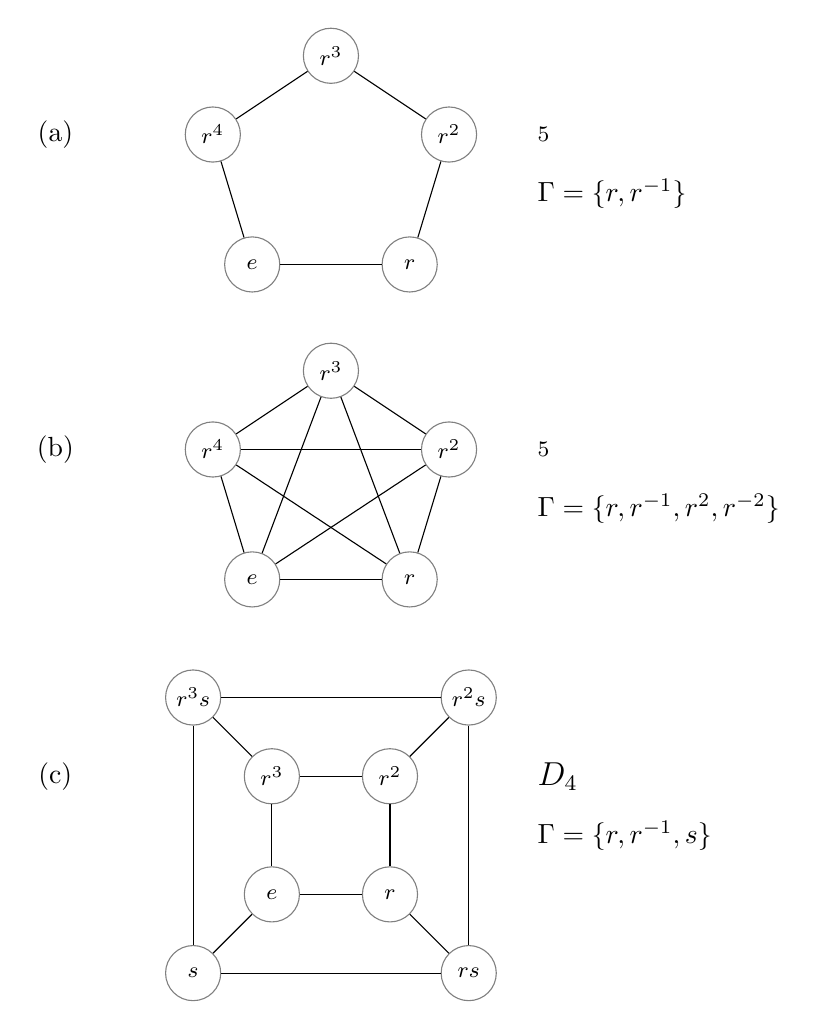
\begin{tikzpicture}[
    cell/.style = {font=\footnotesize, shape=circle, draw=gray, minimum width=0.7cm, inner sep=2pt}
    ]

    \node[cell] (g0) at (0,    0)    {$e$};
    \node[cell] (g1) at (2,    0)    {$r$};
    \node[cell] (g2) at (2.5,  1.65) {$r^2$};
    \node[cell] (g3) at (1,    2.65) {$r^3$};
    \node[cell] (g4) at (-0.5, 1.65) {$r^4$};

    \path [-] (g0) edge (g1);
    \path [-] (g1) edge (g2);
    \path [-] (g2) edge (g3);
    \path [-] (g3) edge (g4);
    \path [-] (g4) edge (g0);

    \begin{scope}[yshift=-4cm]
        \node[cell] (r0) at (0,    0)    {$e$};
        \node[cell] (r1) at (2,    0)    {$r$};
        \node[cell] (r2) at (2.5,  1.65) {$r^2$};
        \node[cell] (r3) at (1,    2.65) {$r^3$};
        \node[cell] (r4) at (-0.5, 1.65) {$r^4$};

        \path [-] (r0) edge (r1);
        \path [-] (r0) edge (r2);
        \path [-] (r1) edge (r2);
        \path [-] (r1) edge (r3);
        \path [-] (r2) edge (r3);
        \path [-] (r2) edge (r4);
        \path [-] (r3) edge (r4);
        \path [-] (r3) edge (r0);
        \path [-] (r4) edge (r0);
        \path [-] (r4) edge (r1);
    \end{scope}

    \begin{scope}[yshift=-8cm, xshift=0.25cm]
        \node[cell] (dih e)   at (0,   0)   {$e$};
        \node[cell] (dih r)   at (1.5, 0)   {$r$};
        \node[cell] (dih r2)  at (1.5, 1.5) {$r^2$};
        \node[cell] (dih r3)  at (0,   1.5) {$r^3$};
        \node[cell] (dih s)   at (-1,  -1)  {$s$};
        \node[cell] (dih rs)  at (2.5, -1)  {$rs$};
        \node[cell] (dih r2s) at (2.5, 2.5) {$r^2s$};
        \node[cell] (dih r3s) at (-1,  2.5) {$r^3s$};

        \path [-] (dih e) edge (dih r);
        \path [-] (dih e) edge (dih s);

        \path [-] (dih e) edge (dih r3);
        \path [-] (dih s) edge (dih r3s);

        \path [-] (dih r) edge (dih r2);
        \path [-] (dih r) edge (dih rs);

        \path [-] (dih r2) edge (dih r3);
        \path [-] (dih r2) edge (dih r2s);

        \path [-] (dih r3) edge (dih r3s);
        \path [-] (dih s) edge (dih rs);

        \path [-] (dih rs) edge (dih r2s);
        \path [-] (dih r2s) edge (dih r3s);
    \end{scope}

    % Group labels
    \node[align=left, anchor=west, font=\large] at (3.5, 1.65) {$\Z_5$};
    \node[align=left, anchor=west, font=\large] at (3.5, -2.35) {$\Z_5$};
    \node[align=left, anchor=west, font=\large] at (3.5, -6.5) {$D_4$};

    % Set labels
    \node[align=left, anchor=west] at (3.5, 0.9) {$\Gamma = \{r, r^{-1}\}$};
    \node[align=left, anchor=west] at (3.5, -3.1) {$\Gamma = \{r, r^{-1}, r^2, r^{-2}\}$};
    \node[align=left, anchor=west] at (3.5, -7.25) {$\Gamma = \{r, r^{-1}, s\}$};

    % Figure labels
    \node[font=\normalsize] at (-2.5, 1.65)  {(a)};
    \node[font=\normalsize] at (-2.5, -2.35) {(b)};
    \node[font=\normalsize] at (-2.5, -6.5)    {(c)};
\end{tikzpicture}

    \caption[Examples of Cayley graphs]{%
        Examples of Cayley graphs.
        (a) and (b) show $\Z_5$ with $\Gamma = \{g,g^{-1}\}$ and $\Gamma = \{g,g^2, g^{-1}, g^{-2}\}$ respectively.
        (c) shows $D_4$ with $\Gamma = \{r,r^{-1}, s\}$
    }
    \label{fig:examples of Cayley graphs}
\end{figure}



\subsubsection{The finite group Laplacian}\label{sec:finitegrouplaplacian}
In this section we explain in detail the construction of the finite group Laplacian, which we take as the electric Hamiltonian, as the graph Laplacian of the Cayley graph of the finite group.
Given a finite group $G$, we choose a set of generators $\Gamma \subset G$, which we require to be invariant under inversion, that is $\Gamma^{-1}=\Gamma$, and moreover that it is the union of conjugacy classes, so that it is invariant under conjugation, $g \Gamma g^{-1}=\Gamma$ for any $g$ in $G$ \cite{spectralgraphtheory}.
We choose $\Gamma$ not to include the identity element and we note that the choice of $\Gamma$ is not unique.
The Cayley graph has the group elements as vertices, and we place an edge between $g \in G$ and $h \in G$ if $h g^{-1} \in \Gamma$.
The result is a simple undirected graph.
Examples of Cayley graphs for the groups $D_4$ and $\Z_5$ are shown in Fig.~\ref{fig:examples of Cayley graphs}.
Given any graph, its Laplacian is defined as \cite{spectralgraphtheory}
\begin{equation}
    L = D-A \ ,
\end{equation}
where $A$ is the adjacency matrix and $D$ is the degree matrix.
Each of these matrices acts on the vector space of graph vertices, which in the case of a Cayley graph can be identified with the group algebra $\C[G]$.
The degree matrix is always diagonal, and in this case $D=\abs{\Gamma} \mathbbm{1}$.
The adjacency matrix $A$ is given by
\begin{equation}
    A_{gh} = \begin{cases}1 & g h^{-1} \in \Gamma\\ 0 & \mathrm{otherwise}\end{cases}
\end{equation}
for group elements $g,h$.
On a basis element, one has
\begin{equation}
    A \ket{g} \equiv \sum_h A_{hg} \ket{h} = \sum_{k \in \Gamma} \ket{gk} = \sum_{k \in \Gamma} \ket{gk^{-1}} = \sum_{k \in \Gamma} R_k \ket{g} \ ,
\end{equation}
where $R_k$ is the right regular representation, and we used the closure of $\Gamma$ under inversion.
Therefore as an operator on $\C[G]$,
\begin{equation}
    A = \sum_{k \in \Gamma} R_k = \bigoplus_j \mathbbm{1}_j \otimes \pqty{\sum_{k \in \Gamma} \rho_j(k)} \ ,
\end{equation}
where we used the Peter-Weyl decomposition of $R_k$, eq.\eqref{eq:translations peter weyl}.
Then we see that
\begin{equation}
    \pqty{\sum_{k \in \Gamma} \rho_j(k)} \rho_j(g) = \sum_{k \in \Gamma} \rho_j(kg) = \sum_{k \in \Gamma} \rho_j((g k g^{-1} g) = \rho_j(g) \pqty{\sum_{k \in \Gamma} \rho_j(k)} \ ,
\end{equation}
where we used the closure of $\Gamma$ under conjugation.
Hence the operator $\pqty{\sum_{k \in \Gamma} \rho_j(k)}$ commutes with the irreducible representation $\rho_j$ and as such is proportional to the identity by Schur's lemma \cite{Serre}.
The constant of proportionality can be readily computed by taking a trace.
This therefore implies
\begin{equation}
    A = \sum_j \lambda_j P_j \ , \quad \quad \lambda_j = \frac{1}{\dim{j}} \sum_{k \in \Gamma} \chi_j(k) \ ,
\end{equation}
where $P_j = \sum_{mn} \ket{jmn}\bra{jmn}$ is the projector onto the $j$th representation subspace, and $\chi_j$ is the character of the irrep labelled $j$.
Therefore the Laplacian of the Cayley graph is given by
\begin{equation}\label{eq:laplacian finite group}
    L = \sum_j f(j) P_j \ , \quad \quad f(j)= \abs{\Gamma}-\frac{1}{\mathrm{dim}(j)} \sum_{k \in \Gamma} \chi_j(k) \ ,
\end{equation}
which is the same form as the electric Hamiltonian in the representation basis, eq.~\eqref{eq:electric hamiltonian rep basis}.

We give some examples of this construction.
For the group $\Z_N$ it is natural to construct the electric eigenvalues $f(j)$ with the generating set $\Gamma = \{g, g^{-1}\}$, which results in
\begin{equation}
    \label{eq:fj ZN}
    f(j)=f(N-j) = 4\sin^2\pqty{\frac{\pi j}{N}} \ ,
\end{equation}
which is the same as in \cite{Ercoetal1}.
Moreover for large $N$,
\begin{equation}
    f(j) \to \frac{4\pi^2}{N^2} j^2\,\,\,\,\,\,\,\,\,\,\,N\,\mathrm{large} \ ,
\end{equation}
which is proportional to the Casimir eigenvalues of the $\U(1)$ gauge theory \cite{Ercoetal2}.
Thus both a truncation of $\U(1)$ theory and proper $Z_N$ gauge theory naively approach $\U(1)$ theory for large $N$, albeit in different ways.
One can however choose a different generating set, such as $\Gamma = \{g, g^{-1},g^2, g^{-2}\}$ and the corresponding eigenvalues would be
\begin{equation}
    f(j)=f(N-j) = 4\sin^2\pqty{\frac{\pi j}{N}}+4\sin^2\pqty{\frac{2\pi j}{N}} \ .
\end{equation}
For the dihedral group $D_4$ we can choose for example $\Gamma = \Gamma_1 = \{r,r^3,s,r^2s\}$, which gives rise to the eigenvalues $f(j)$  shown in table \ref{tab:fval}, where the representations are ordered like in the character table in Table \ref{tab:chars_D4} in Appendix \ref{app:the_dihedral_groups}.
Note that $\Gamma_1$ generates the whole group.

\begin{table}[t]
    \centering
    \begin{tabular}{rcccccc}
        \toprule
         & & \multicolumn{5}{c}{$f(j)$} \\
        \cmidrule(l){3-7}
        $\Gamma$~~~ & $j$ & 0 & 1 & 2 & 3 & 4\\
        \midrule
        $\{r, r^3, s, r^2 s \}$
                 & & 0 & 4 & 4 & 8 & 4 \\[5pt]
        $\{r, r^2, r^3 \}$
                 & & 0 & 4 & 0 & 4 & 5 \\[5pt]
        $\{r, r^3, s, r s, r^2 s, r^3 s \}$
                       & & 0 & 8 & 8 & 8 & 6 \\
        \bottomrule
    \end{tabular}
    \caption{Eigenvalues of the single-link electric Hamiltonian $f(j)$ for the finite group $D_4$, with three choices of generating sets $\Gamma$.}
    \label{tab:fval}
\end{table}


By looking at its character table, we may in fact classify all possible choices of $\Gamma$ for $D_4$.
In fact, $D_4$ has five conjugacy classes, $C_0 = \{e\}$, $C_1 = \{r, r^3\}$, $C_2 = \{r^2\}$, $C_3 = \{s, r^2s\}$, $C_4 = \{rs, r^3s\}$.
One can check that, as is generally true, $\sum_i \abs{C_i}=8=\abs{G}$.
In this case, all conjugacy classes are invariant under inversion, i.e.
$C_i^{-1}=C_i$.
 Hence any union of the $C_i$s, $i \neq 0$ is a valid choice for $\Gamma$.
There are $2^4$ such possibilities.
Note that this is not true in general, in which case one must choose conjugacy classes to ensure that $\Gamma^{-1}=\Gamma$.
We consider in more detail two specific cases, in particular $\Gamma_2 = C_1 \cup C_2 = \{r, r^2, r^3\}$.
Unlike $\Gamma_1$, $\Gamma_2$ does not generate the whole group $D_4$; this is reflected in the electric eigenvalues in Table \ref{tab:fval}, with the ground state being two-fold degenerate.
Finally, we consider the choice $\Gamma_3=C_1 \cup C_3 \cup C_4=\{r, r^3, s, rs, r^2s, r^3s\}$.
As explained in Section \ref{sec:action formulation} if we pick $h_B$ as the real part of the trace of the two-dimensional representation of $D_4$, the choice of $\Gamma_3$ corresponds to the Lorentz-invariant Hamiltonian.

\subsubsection{Action formulation and Lorentz invariance}\label{sec:action formulation}

The Kogut-Susskind Hamiltonian eq.~\eqref{eq:kog suss hE hB} may be obtained via the transfer-matrix formulation from the Euclidean Wilson action \cite{CreutzTransferMatrix,KogRev}
\begin{equation}
    \label{eq:wilson action}
    S = -\frac{1}{g^2 a^{4-d}} \sum_{\square} \Re \tr{\rho(g_\square)} \ ,
\end{equation}
where $a$ is the lattice spacing and $g$ the coupling.
The couplings in  eq.~\eqref{eq:kog suss hE hB} also take the specific form $\lambda_E = \frac{g^2}{2a^{d-2}}$ and $\lambda_B = \frac{2}{g^2 a^{4-d}}$.
In the path-integral formulation, the lattice is fully discretized and thus plaquettes extend also in the time direction.
The action eq.~\eqref{eq:wilson action} is also perfectly valid for finite groups, as one simply replaces the partition function integration measure over the Lie group with sum over the elements of a finite group.
One may then repeat the transfer-matrix formulation for an arbitrary finite group \cite{TransferMatrixFiniteGroup}.
The resulting finite group Hamiltonian takes the form eq.~\eqref{eq:generalized ym hamiltonian}, with specific choices of $\Gamma$ and $h_B$.
In particular, $h_B$ is chosen as usual like in eq.~\eqref{eq:kog suss hE hB}, while $\Gamma = \{g \in G,\,\, g \neq e, \mathrm{max} \bqty{\Re \tr{\rho(g)}}  \}$ is the set of non-identity elements which maximize $\Re \tr{\rho(g)}$.
More generally, one may start from a Euclidean action of the form
\begin{equation}
    \label{eq:anisotropic action}
    S = -\sum_{\square_t} f_t(g_{\square_t}) - \sum_{\square_s} f_s(g_{\square_s}) \ ,
\end{equation}
where $\square_t$ and $\square_s$ are plaquettes in the time and space directions respectively, and $f_t, f_s$ are real functions such that $f(g_1 g_\square g_1^{-1})=f(g_\square)$ for any $g_1 \in G$.
Then via the transfer matrix procedure one obtains a generalized Hamiltonian of the form of eq.~\eqref{eq:generalized ym hamiltonian} with $h_B = f_s$ and $\Gamma = \{g \in G,\,\, g \neq e, \mathrm{max} \bqty{f_t(g)} \}$.
Even though we do not consider this case here, in order to improve the approach to the continuum it might also be interesting to consider other Euclidean actions \cite{Hasenfratz1,LammChairs}.

In particle physics applications, one typically requires Lorentz invariance in the continuum.
While the lattice breaks the Lorentz symmetry to the subgroup of Euclidean cubic rotations, as long as this subgroup is preserved one expects to recover Lorentz invariance in the continuum limit.
Since the action eq.~\eqref{eq:anisotropic action} is anisotropic in the space and time directions, it breaks the Euclidean cubic symmetry explicitly and it is unclear whether the corresponding Hamiltonian describes a Lorentz-invariant theory in the continuum (unless of course $f_s=f_t$).
This includes in particular setting $h_E(j)=j^2$ for subgroups of $\U(1)$ and $h_E(j)=j(j+1)$ for subgroups of $\SU(2)$ in eq.~\eqref{eq:electric hamiltonian rep basis}, while keeping $h_B$ unchanged.
Such choices explicitly break the remnant Lorentz symmetry.
In condensed matter applications, however, Lorentz invariant is not necessarily required and one may thus independently choose $\Gamma$ and $h_B$, as well as the couplings $\lambda_E$ and $\lambda_B$.


\subsubsection{Classification of the possible theories, and other models}\label{sec:classification}

The construction of finite group Yang-Mills gauge theories with Hamiltonian eq.~\eqref{eq:generalized ym hamiltonian} involves a few arbitrary choices which can be classified.
Since the Hilbert space is fixed to the physical, gauge-invariant Hilbert space $\mathcal{H}_{\mathrm{phys}}$, the only possible choices involve the various terms in the Hamiltonian.
Given a gauge group $G$ in $d$ spatial dimensions, one may arbitrarily choose:
\begin{enumerate}
    \item A set $\Gamma$ of group elements which does not contain the identity, and is invariant under both inversion and conjugation $\Gamma^{-1}=\Gamma$ and $g \Gamma g^{-1}$.

    \item A choice for the magnetic Hamiltonian $h_B = h_B(g_\square)$.
Since it must be real and satisfy $h_B(g_1 g_\square g_1^{-1})= h_B(g_\square)$, i.e.
it is a \textit{class function}, by a well-known result \cite{Serre} it may be expanded in a sum of characters of irreducible representations, $h_B(g) = \sum_j c_j \chi_j(g)$ for coefficients $c_j$ which may be chosen arbitrarily, while ensuring that $h_B(g)$ is real.
    \item If present, possible choices of representations and Hamiltonians in the matter sector.
For example in $D_4$ gauge theory, one can include \textit{staggered fermions} in the two-dimensional representation.

    \item One can also add a Chern-Simons term as in \cite{Caspar_Wiese}.
This is especially interesting for \ac{qs}, because such theories have a sign problem.
\end{enumerate}
Further considerations involve the Lorentz symmetry, as explained in Section \ref{sec:action formulation}.
Moreover, one may want to choose representations which are non-trivial when restricted to the center of the gauge group \cite{CenterSymmetry, Cohen_2014}.

We note that the above construction allows further generalizations.
In particular, the discretized $d$-dimensional space does not have to take the form of a hypercubic lattice, but more generally can be a Bravais or non-Bravais lattice.
No difference arises for the electric term, which is link-based, and the plaquette variable in the magnetic term is replaced by an an elementary closed loop in the lattice.


%The finite-group Yang-Mills theories may also be compared with another %type of finite group gauge theories known as Quantum Double Models. %These are defined on the same overall Hilbert space $\mathcal{H} = %\bigotimes_{\mathrm{links}} \C[G]$, but one does not impose the Gauss' %law constraint eq.~\eqref{eq:lattice gauss law} and thus all states %are allowed. The Hamiltonian is different; the electric  is chosen to %be the Gauss' law operator on each vertex, while the magnetic term is %chosen to be $h_B(g_\square) = \delta(g_\square,1)$. For Quantum %Double Models, the electric and magnetic Hamiltonians commute with %each other and thus the physics of the theory is rather different from %that of the models we're considering. In the limit where %$\lambda_E=0$, however, the ground state of a Quantum Double Model coincides with the ground state of the finite group Yang-Mills %theory with the same gauge group $G$ and the same magnetic term $h_B$.




% SECTION: The physical Hilbert space
% \section{The physical Hilbert space}\label{sec:physical Hilbert space}

As we remarked in Sec.~\ref{sec:from_lie_groups_to_finite_groups}, while the overall Hilbert space of the pure gauge theory is $\mathcal{H} = \bigotimes_{\mathrm{links}} \C[G]$, only those states that satisfy the so-called \say{Gauss' law} constraint \eqref{eq:lattice gauss law} are to be considered physical \cite{kogut1975hamiltonian, milstead2018qyangmills, tong2018gauge}.
For gauge theories based on most compact Lie groups, the \ac{wl}s (despite being overcomplete) span the space of gauge-invariant states \cite{Sengupta, Durhuus}.
This, however, is not necessarily true for finite groups \cite{Sengupta, Cui}; this means that in some cases, it is possible to construct different gauge-invariant states, which nevertheless have the identical \ac{wl}s.
We mention that this difficulty cannot arise for Abelian finite groups such as $\Z_N$, in which case the \ac{wl}s \textit{do} span the physical Hilbert space $\mathcal{H}_{\mathrm{phys}}$.
In the following section we give a description of the gauge-invariant Hilbert space in terms of \textit{spin network states} and explain how this basis of states is particularly suitable to describe the physical Hilbert space of finite group gauge theories.
We first consider the pure gauge physical Hilbert space in Section \ref{sec:spin networks pure gauge} and compute its dimension in Section \ref{sec:spin networks dimension}.
% In Section \ref{sec:spin networks matter} we extend this construction to matter fields.

\subsection{Spin networks}\label{sec:spin networks pure gauge}

The physical Hilbert space of pure gauge theories with either Lie or finite gauge group can be explicitly described in terms of \textit{spin network states} \cite{Baez, Burgio}.
Spin-network states can be defined indifferently when the $d$-dimensional space is discretized as an arbitrary graph, and are thus valid in arbitrary dimension with arbitrary lattices and boundary conditions.
The first key observation is that the action of the Gauss' law operator eq.~\eqref{eq:lattice gauss law} is block-diagonal in the representation basis, as can be seen from eq.~\eqref{eq:translations peter weyl}.
Then starting from the Hilbert space in the representation basis eq.~\eqref{eq:peterweyl}, we can, as usual, permute the summation and product, obtaining
\begin{equation}
    \label{eq:hilbert space permuted}
    \mathcal{H} = \bigotimes_{\mathrm{links}} \bigoplus_{j \in \Sigma} V_j^* \otimes V_j=\bigoplus_{\{j\} \in \{\Sigma\}} \bigotimes_{l \in \mathrm{links}}  V_{j_l}^* \otimes V_{j_l} \ ,
\end{equation}
where now $\{j\}$ is an assignment of an irrep $j_l$ to each lattice link $l$, and $\{\Sigma\}$ is the set of the possible such assignments.
The second key observation is that the gauge transformations eq.~\eqref{eq:lattice gauss law} are given by an independent group-valued variable $g_x$ at each site $x$ of the lattice.
Moreover, due to eq.~\eqref{eq:translations peter weyl} the gauge transformation associated to one site $x$ acts at most on one of $V_j$ or $V_j^*$ but it cannot act on both.
One can then split the two vector spaces $V_j$ and $V_j^*$ associated with each link and reorder the $V$s in the tensor product over links so that $V_j$s are now grouped together according to the \textit{sites} and not the links,
\begin{equation}
    \mathcal{H} = \bigoplus_{\{j\} \in \{\Sigma\}} \bigotimes_{x \in \mathrm{sites}} \pqty{\bigotimes_{l_-=x} V_{j_l}^*} \otimes \pqty{\bigotimes_{l_+=x} V_{j_l} }\ ,
\end{equation}
where by $l_+$ and $l_-$ we denote respectively the target and source vertex of link of link $l$.
We can repeat the same set of operations for the gauge transformation operator eq.~\eqref{eq:gauss law operator}, which are therefore given by
\begin{equation}
    \mathcal{G}(\{g_x\}) = \bigoplus_{\{j\} \in \{\Sigma\}} \bigotimes_{x \in \mathrm{sites}} \pqty{\bigotimes_{l_-=x} \rho_{j_l}^*(g_x)} \otimes \pqty{\bigotimes_{l_+=x} \rho_{j_l}(g_x) }\ .
\end{equation}
In the above decomposition, the gauge transformations now act independently for each $x$ and the Gauss' law constraint EQ.~\eqref{eq:lattice gauss law} gives the physical Hilbert space
\begin{equation}
    \label{eq:spin network Hilbert space}
    \mathcal{H}_{\mathrm{phys}} = \bigoplus_{\{j\} \in \{\Sigma\}} \bigotimes_{x \in \mathrm{sites}} \mathrm{Inv}\bqty{\pqty{\bigotimes_{l_-=x} V_{j_l}^*} \otimes \pqty{\bigotimes_{l_+=x} V_{j_l} }} \ .
\end{equation}


\begin{figure}[t]
    \SideFigure[label=fig:periodic plaquette, desc={Links on the $2 \times 2$ lattice}]{%
        \begin{tikzpicture}[
        testo/.style={midway, black},
        inside link/.style = {very thick, Grey80, ->-=0.5},
        outside link/.style = {very thick, Grey80, ->-=0.5, dashed}
        ]
    \draw[inside link]  (0,0) -- (2,0) node[testo, below] {$\link_1$};
    \draw[inside link]  (2,0) -- (2,2) node[testo, right] {$\link_2$};
    \draw[inside link]  (0,2) -- (2,2) node[testo, above] {$\link_3$};
    \draw[inside link]  (0,0) -- (0,2) node[testo, left ] {$\link_4$};
    \draw[outside link] (0,2) -- (0,4) node[testo, left ] {$\link_8$};
    \draw[outside link] (2,2) -- (2,4) node[testo, right] {$\link_7$};
    \draw[outside link] (2,2) -- (4,2) node[testo, above] {$\link_6$};
    \draw[outside link] (2,0) -- (4,0) node[testo, below] {$\link_5$};
    \DrawSites{0,2}{0,2};

    \begin{scope}[xshift=6cm, yshift=2cm]
        \draw[inside link] (0, 0) -- (2, 0) node [testo, above] {$\link$};
        \node[site, label=below:{$\link_-$}] at (0, 0) {};
        \node[site, label=below:{$\link_+$}] at (2, 0) {};
    \end{scope}
\end{tikzpicture}

    }{%
    A $2\times 2$ square lattice with periodic boundary conditions, showing the labels of the links.
    }
\end{figure}

Given a representation $\rho$ (not necessarily irreducible) with representation space $V_\rho$, the set of invariant vectors $\mathrm{Inv}(V_\rho)$ is the set of vectors $v \in V_\rho$ such that $\rho(g) v = v$ for all $g\in G$.
Note that this is a separate notion from that of an \say{invariant subspace}.
A basis of \textit{spin network states} which arise from the description of eq.~\eqref{eq:spin network Hilbert space} are of the form $\ket{\{j\},A}$ where $\{j\}$ is an assignment of irreps to links and $A=(a_1, \ldots a_V)$ labels the choice of a gauge-invar


For a hypercubic lattice in $d$ dimensions with periodic boundary conditions, each site is connected to $2d$ links and therefore $2d$ terms appear in the tensor product within each $\mathrm{Inv}$ in eq.~\eqref{eq:spin network Hilbert space}.
If instead we choose open boundary conditions, the sites in the bulk will again be connected to $2d$ links, but the sites on the boundary will be connected to fewer links and thus fewer terms will appear in the tensor product for those sites.
In the general case, the number of terms in the tensor product within each $\mathrm{Inv}$ may depend on the site.
We choose to work directly with the spaces of invariant vectors rather than with spaces of intertwiners more commonly employed in the literature \cite{Baez, Burgio}.

The calculation of a basis of invariant states (or, equivalently, of the intertwiners) can be difficult in the Lie group case, especially since they admit infinitely many irreps, but can quite easily be performed numerically for finite groups, which only have finitely many irreps.
Since the number of links connected to each site is finite and independent of the lattice volume, one needs only compute the invariant states of a finite number of tensor product representations which does not scale with the lattice size.

As an example, we work out explicitly the case of a $2\times 2$ square lattice with periodic boundary conditions.
As shown in Fig.~\ref{fig:periodic plaquette}, this system has four vertices and eight links.
Expanding explicitly eq.~\eqref{eq:spin network Hilbert space} we see that in this case
\begin{align}
    \mathcal{H}_{\mathrm{phys}} &= \bigoplus_{j_1, \ldots j_8}
    \mathrm{Inv}\bqty{V_{j_1}^* \otimes V_{j_4}^* \otimes V_{j_5} \otimes V_{j_8}} \otimes
    \mathrm{Inv}\bqty{V_{j_5}^* \otimes V_{j_2}^* \otimes V_{j_1} \otimes V_{j_7}}  \otimes \\
    &\quad\otimes\mathrm{Inv}\bqty{V_{j_6}^* \otimes V_{j_7}^* \otimes V_{j_3} \otimes V_{j_2}} \otimes
    \mathrm{Inv}\bqty{V_{j_3}^* \otimes V_{j_8}^* \otimes V_{j_6} \otimes V_{j_4}} \ . \nonumber
\end{align}
Now consider a single invariant subspace $\mathrm{Inv}\bqty{V_{j_1}^* \otimes V_{j_2}^* \otimes V_{j_3} \otimes V_{j_4}}$ with arbitrary assignment of representations.
This vector space admits an orthonormal basis $\{\ket{j_1 j_2 j_3 j_4 ; a}\}$ where $1 \leq a \leq \dim\mathrm{Inv}\bqty{V_{j_1}^* \otimes V_{j_2}^* \otimes V_{j_3} \otimes V_{j_4}}$ indexes the basis vector.
We can expand the basis vectors explicitly in terms of the bases of the $V_j$ as (see also the discussion around eq.~\eqref{eq:change of basis})
\begin{equation}
    \ket{j_1 j_2 j_3 j_4 ; a} = \sum_{m_1, m_2, n_3, n_4} \psi\pqty{j_1 m_1 j_2 m_2 j_3 n_3 j_4 n_4 ; a} \ket{j_1 m_1} \otimes \ket{j_2 m_2} \otimes \ket{j_3 n_3} \otimes \ket{j_4 n_4} \ .
\end{equation}
The basis vectors can be chosen orthonormal.
By virtue of spanning the space $\mathrm{Inv}\bqty{V_{j_1}^* \otimes V_{j_2}^* \otimes V_{j_3} \otimes V_{j_4}}$, they are invariant vectors of the tensor product representation $\rho \equiv \rho_{j_1}^* \otimes \rho_{j_2}^* \otimes \rho_{j_3} \otimes \rho_{j_4}$; as such, they satisfy $\rho(g) \ket{j_1 j_2 j_3 j_4 ; a} = \ket{j_1 j_2 j_3 j_4 ; a}$ for all $g \in G$.
The coefficients of the expansion $\psi\pqty{j_1 m_1 j_2 m_2 j_3 n_3 j_4 n_4 ; a}$ may be easily computed, for example by writing the tensor product representation matrices $\rho(g)$ explicitly and then solving the simultaneous equations $\rho(g) v = v$ for all $g \in G$ (it is actually sufficient to do so on a set of generators of $G$).
The dimension of the space of invariant vectors depends on the four representations assigned to the relevant site.
Now let $A = \pqty{a_1, a_2, a_3, a_4}$, which implicitly depends on $\{j\}$ (because the range of each $a_i$ depends on the irreps assigned to site $i$).
Given any assignment of irreps $\{j\}$, $A$ is a choice of a basis vector of invariant states at the four sites.
Therefore an orthonormal basis for the gauge invariant Hilbert space is given by
\begin{equation}
    \ket{ \{j\};A} = \ket{j_1 j_4 j_5 j_8 ; a_1} \otimes \ket{j_5 j_2 j_1 j_7 ; a_2} \otimes \ket{j_6 j_7 j_3 j_2 ; a_3} \otimes \ket{j_3 j_8 j_6 j_4 ; a_4} \ ,
\end{equation}
for any possible assignment $\{j\}$ of irreps to links, and then all possible choices $A$ of an invariant vector at each of the four sites.

The spin-network states $\ket{ \{j\};A}$ then form a basis of the gauge-invariant Hilbert space.
Expanding the tensor product, we find an explicit expression for these states in terms of the representation basis,
\begin{align}
    \ket{ \{j\};A} &= \sum_{n_1, \ldots n_8} \sum_{m_1, \ldots m_8} \psi\pqty{j_1 m_1 j_4 m_4 j_5 n_5 j_8 n_8 | a_1} \psi\pqty{j_5 m_5 j_2 m_2 j_1 n_1 j_7 n_7 | a_2} \times \\
    &\quad \quad \times \psi\pqty{j_6 m_6 j_7 m_7 j_3 n_3 j_2 n_2 | a_3} \psi\pqty{j_3 m_3 j_8 m_8 j_6 n_6 j_4 n_4 | a_4} \times \\
    &\quad \quad \times \ket{j_1 m_1 n_1} \otimes \ket{j_2 m_2 n_2} \otimes \cdots \ket{j_8 m_8 n_8} \ ,
\end{align}
where we have restored the ordering of the vector spaces $V_j$s and used again the shorthand $\ket{jmn}=\ket{jm}\otimes \ket{jn}$.
We note in particular that despite having introduced a splitting of the variables at each link, in the final answer this splitting disappears and the spin-network states can be entirely expressed in terms of the representation basis $\ket{jmn}$.

\subsection{The dimension of the physical Hilbert space}\label{sec:spin networks dimension}

As we have seen in the previous section, spin network states give an explicit description of the physical Hilbert space $\mathcal{H}_{\mathrm{phys}}$ as
\begin{equation}
    \mathcal{H}_{\mathrm{phys}} =\bigoplus_{\{\rho\} \in \{\Sigma\}} \bigotimes_{v \in \mathrm{sites}} \mathrm{Inv}\bqty{\pqty{\bigotimes_{l_- = v}  V_{\rho_l}^*} \otimes \pqty{\bigotimes_{l_+ = v}  V_{\rho_l}}} \ ,
\end{equation}
where $\mathrm{Inv}(\rho)$ is the space of invariant vectors of the representation $\rho$, $\{\rho\}$ is an assignment of irreps to links and $\{\Sigma\}$ is the set of such possible assignments.
For a finite group,
\begin{equation}
    \label{eq:invariant vectors counting}
    \dim{\mathrm{Inv}(\rho)} = \frac{1}{\abs{G}} \sum_{g \in G} \chi_\rho(g) \ ,
\end{equation}
where $\chi_\rho$ is the character of $\rho$.
We prove this result in Appendix \ref{sec:counting invariant states}.
This fact can be used to obtain a general formula for the dimension of the $\mathcal{H}_{\mathrm{phys}}$, which is valid for any lattice in any dimension with any boundary conditions.
On a lattice with $L$ links and $V$ sites, we will show that
\begin{equation}
    \label{eq:physical hilbert space dimension}
    \dim{\mathcal{H}_{\mathrm{phys}}} = \sum_C \pqty{\frac{\abs{G}}{\abs{C}}}^{L-V} \ ,
\end{equation}
where the sum runs over all conjugacy classes $C$ of the group, and $\abs{C}$ is the size of $C$.
The ratio $\abs{G}/\abs{C}$ is always an integer by the orbit-stabilizer theorem \cite{Serre}.
Using eq.\eqref{eq:invariant vectors counting}, together with the fact that the character of a tensor product is given by the product of the characters, we may readily prove eq.\eqref{eq:physical hilbert space dimension}.
From the general formula for the gauge-invariant Hilbert space, we have
\begin{align}
    \dim{\mathcal{H}_{\mathrm{phys}}} &=\sum_{j_1 j_2 \cdots j_L} \prod_{v \in \mathrm{sites}} \dim\mathrm{Inv}\bqty{\pqty{\bigotimes_{l_- = v}  V_{\rho_l}^*} \otimes \pqty{\bigotimes_{l_+ = v}  V_{\rho_l}}} = \nonumber \\
    &=\frac{1}{\abs{G}^V}\sum_{j_1 j_2 \cdots j_L} \sum_{g_1 g_2 \cdots g_V} \prod_{v \in \mathrm{sites}} \pqty{\prod_{l_- = v}  \chi_{j_l}^*(g_v)}  \pqty{\prod_{l_+ = v} \chi_{j_l}(g_v)} \nonumber \ .
\end{align}
Within the product over all sites, there are exactly $2L$ factors of characters $\chi$, as each link contributes two representation spaces $V$ and each representation space gives rise to a character.
Thus grouping characters by link, we obtain
\begin{equation}
    \dim{\mathcal{H}_{\mathrm{phys}}} =\frac{1}{\abs{G}^V} \sum_{g_1 g_2 \cdots g_V} \prod_{l = \expval{xx'} \in \mathrm{links}} \expval{g_x, g_{x'}} \ .
\end{equation}
where we denoted $\expval{g, h} = \sum_j \chi_j(g)^* \chi_j(h)$.
It is a well-known result that $\expval{g, h}$ is zero unless $g$ and $h$ belong to the same conjugacy class, in which case $\expval{g, h} = \abs{G} / \abs{C}$ where $C$ is the conjugacy class of both $g$ and $h$ \cite{Serre}.
If any two adjacent sites $x$ and $x'$ have $g_x$ and $g_{x'}$ in different conjugacy classes, then $\expval{g_x, g_{x'}}=0$ and the corresponding term in the sum is zero.
Assuming that the lattice is connected, this implies that the product over all links is zero unless all the $g_x$ at each site $x$ belong to the same conjugacy class.
Then, since $\expval{g_x, g_{x'}}$ is constant on conjugacy classes, we can write
\begin{equation}
    \dim{\mathcal{H}_{\mathrm{phys}}}
    =\frac{1}{\abs{G}^V} \sum_C \sum_{g_1 g_2 \cdots g_V \in C} \frac{\abs{G}^L}{\abs{C}^L} = \sum_C  \pqty{\frac{\abs{G}}{\abs{C}}}^{L-V} \ ,
\end{equation}
which concludes the proof.
In the Abelian case the above formula simplifies as all conjugacy classes are singlets and therefore $\dim{\mathcal{H}_{\mathrm{phys}}} = \abs{G}^{L-V+1}$.
Thus finite Abelian groups have the largest physical Hilbert space among all groups of the same order.
For periodic boundary conditions in a hypercubic lattice, $L=Vd$ and as such $\dim{\mathcal{H}}=\abs{G}^{Vd}$, while $\dim{\mathcal{H}_{\mathrm{phys}}} \approx \abs{G}^{V (d-1)}$, so that $\dim{\mathcal{H}_{\mathrm{phys}}} \approx (\dim{\mathcal{H}})^{1-1/d}$ and both spaces grow exponentially with the lattice size.
For a finite group, one may compute all possible relevant spaces of invariant vectors with little effort as the number of tensor product spaces is bounded in $d$ spatial dimensions by $\pqty{\dim{j}_\mathrm{max}}^{2d} \leq \abs{G}^d$, owing to $\sum_j \pqty{\dim{j}}^2 = \abs{G}$, independently from the lattice volume.
The exponential scaling arises from considering all possible assignments of irreps to lattice links.

As a further example, we consider the dimension of the Hilbert space for pure $D_4$ gauge theory.
Using eq.~\eqref{eq:physical hilbert space dimension}, we find for $G=D_4$ on a lattice with $L$ links and $V$ sites,
\begin{equation}
    \dim{\mathcal{H}_{\mathrm{phys}}} = 8^{L-V}\pqty{2+\frac{3}{2^{L-V}}} \ .
\end{equation}
The dimension of the physical Hilbert space for some two-dimensional finite square lattices in $2+1$ dimensions is shown in Table \ref{tab:numstates}.
We see that its size grows quickly with the lattice size.
We point out that even for a $2 \times 2$ periodic lattice with a small group such as $D_4$ it is not even feasible to write down all possible gauge-invariant states.
Unless the structure happens to be very sparse, writing down the $8960$ physical basis elements in terms of the $\abs{G}^L = 8^8$ basis elements in the representation basis using $4 \mathrm{B}$ floating point numbers would require roughly $600 \mathrm{GB}$ of memory.
\begin{table}[t]
    \centering
    \begin{tabular}{clrrcr}
        \toprule
        Size~~~ & BCs & $L$ & $V$ & $L-V$ &$\dim{\mathcal{H}_{\mathrm{phys}}}$\\
        \midrule
        \multirow{2}{3em}{$2 \times 2$}
            & open & $4$ & $4$ & $0$ & $5$\\
            & periodic & $8$ & $4$ & $4$ & $8960$ \\[5pt]
        \multirow{2}{3em}{$2 \times 3$}
            & open & $7$ & $6$ & $1$ & $28$ \\
            & periodic & $12$ & $6$ & $6$ & $536576$ \\[5pt]
        \multirow{2}{3em}{$3 \times 3$}
            & open & $12$ & $9$ & $3$ & $1216$ \\
            & periodic & $18$ & $9$ & $9$ & $269221888$ \\
        \bottomrule
    \end{tabular}
    \caption{Dimension of the physical subspace of $D_4$ gauge theory on some small lattices in $2+1$ dimensions.
$L$ is the number of links and $V$ is the number of vertices.}
    \label{tab:numstates}
\end{table}

% \subsection{Extension to matter fields} \label{sec:spin networks matter}
%
% The spin network states may be extended to matter


\newcommand{\InvSpace}[4]{\mathrm{Inv}\bqty{ V_{j_{#1}}^{\ast} \otimes V_{j_{#2}}^{\ast} \otimes V_{j_{#3}} \otimes V_{j_{#4}}}}
\newcommand{\jm}[1]{\ket{j_{#1} m_{#1}}}
\newcommand{\jn}[1]{\ket{j_{#1} n_{#1}}}
\newcommand{\jmn}[1]{\ket{j_{#1} m_{#1} n_{#1}}}

\section{The physical Hilbert space}\label{sec:physical Hilbert space}

As we remarked in Sec.~\ref{sub:the_hilbert_space}, while the overall Hilbert space of the pure gauge theory is $\HilbertTot = \bigotimes_{\link} \HilbertG_{\link}$, only those states that satisfy the so-called ``Gauss' law'' constraint \eqref{eq:lattice gauss law} are to be considered physical \cite{kogut1975hamiltonian, milstead2018qyangmills, tong2018gauge}.

For gauge theories based on most compact Lie groups, the Wilson loops (despite being overcomplete) span the space of gauge-invariant states \cite{sengupta1994gaugeinvariant, durhuus1980gaugeinvariant}.
This, however, is not necessarily true for finite groups \cite{sengupta1994gaugeinvariant, cui2020kitaev}; this means that in some cases, it is possible to construct different gauge-invariant states, which nevertheless have identical Wilson loops.
We mention that this difficulty does not arise for Abelian finite groups such as $\Z_N$, in which case the Wilson loops \emph{do} span the physical Hilbert space $\HilbertPhys$.

As will be discussed in Sec.~\ref{sec:spin networks pure gauge}, the gauge-invariant Hilbert space for pure gauge theories may be described in terms of \emph{spin network states}. This basis turns out to be particularly suitable for finite gauge groups and in Sec.~\ref{sub:dimension_physical_hilbert_space} we give a simple formula to compute the dimension of the physical Hilbert space for any finite gauge group.

\subsection{Spin network states}\label{sec:spin networks pure gauge}

The physical Hilbert space of pure gauge theories with either Lie or finite gauge group can be explicitly described in terms of \emph{spin network states} \cite{baez1996spinnetworks, burgio2000physical}.
Spin network states can be defined indifferently when the $d$-dimensional space is discretized as an arbitrary graph, and are thus valid in arbitrary dimension with arbitrary lattices and boundary conditions.

\medskip

The first key observation is that the action of the Gauss' law operator \eqref{eq:lattice gauss law} is block-diagonal in the representation basis, as can be seen from \eqref{eq:translations peter weyl}.
Then starting from the Hilbert space in the representation basis \eqref{eq:peterweyl}, we can, as usual, permute the summation and product, obtaining
\begin{equation}
    \label{eq:hilbert space permuted}
    \HilbertTot =
    \bigotimes_{\Lattice} \bigoplus_{j \in \Sigma} V_j^* \otimes V_j =
    \bigoplus_{\{j\} \in \{\Sigma\}} \bigotimes_{\link \in \Lattice}  V_{j_{\link}}^* \otimes V_{j_{\link}}.
\end{equation}
where now $\{j\}$ is an assignment of an irrep $j_{\link}$ to each lattice link $\link$, and $\{\Sigma\}$ is the set of the possible assignments.
The second key observation is that the gauge transformations \eqref{eq:lattice gauss law} are given by an independent group-valued variable $g_x$ at each site $x$ of the lattice.

Moreover, due to \eqref{eq:translations peter weyl} the gauge transformation associated to one site $x$ acts at most on one of the spaces $V_j$ or $V_j^*$ associated to a link, but it cannot act on both.
One can then split the two vector spaces $V_j$ and $V_j^*$ associated with each link and reorder the $V$'s in the tensor product over links so that $V_j$'s are now grouped together according to the \emph{sites} $x \in \Lattice$ and not the links,
\begin{equation}
    \HilbertTot =
    \bigoplus_{\{j\} \in \{\Sigma\}} \bigotimes_{x \in \Lattice} \pqty{\bigotimes_{\link_{-}=x} V_{j_{\link}}^*} \otimes \pqty{\bigotimes_{\link_{+}=x} V_{j_{\link}} }\ ,
\end{equation}
where by $\link_{+}$ and $\link_{-}$ we denote respectively the target and source vertex of link $\link$ (see Fig.~\ref{fig:periodic plaquette}).

\medskip

We can repeat the same set of operations for the gauge transformation operator \eqref{eq:gauss law operator}, which is therefore given by
\begin{equation}
    \mathcal{G}(\{g_x\}) =
    \bigoplus_{\{j\} \in \{\Sigma\}} \bigotimes_{x \in \Lattice} \pqty{\bigotimes_{\link_{-}=x} \rho_{j_{\link}}^*(g_x)} \otimes \pqty{\bigotimes_{\link_{+}=x} \rho_{j_{\link}}(g_x) }.
\end{equation}
In the above decomposition, the gauge transformations now act independently for each $x$ and the Gauss' law constraint \eqref{eq:lattice gauss law} gives the physical Hilbert space
\begin{equation}
    \label{eq:spin network Hilbert space}
    \HilbertPhys = \bigoplus_{\{j\} \in \{\Sigma\}} \bigotimes_{x \in \Lattice} \mathrm{Inv}\bqty{\pqty{\bigotimes_{\link_{-}=x} V_{j_{\link}}^*} \otimes \pqty{\bigotimes_{\link_{+}=x} V_{j_{\link}} }}.
\end{equation}
Given a representation $\rho$ (not necessarily irreducible) with representation space $V_\rho$, the \emph{set of invariant vectors} $\mathrm{Inv}(V_\rho)$ is the set of vectors $v \in V_\rho$ such that $\rho(g) v = v$ for all $g\in G$.
Note that this is a \emph{separate notion} from that of an ``invariant subspace''.
The characterization of the Hilbert space \eqref{eq:spin network Hilbert space} implies that any physical, gauge-invariant state $\ket{\Psi}$ (i.e.
a state which satisfies the Gauss' law \eqref{eq:lattice gauss law}) may be expanded in a basis of \emph{spin network states},
\begin{equation}
    \ket{\Psi} = \sum_{ \{j\} } \sum_{ A } \Psi(\{j\}; A) \ket{\{j\},A}, \qquad \ket{\{j\},A} = \bigotimes_{x \in \Lattice} \ket{\{j\}_x,a_x},
\end{equation}
where $\{j\}$ is an assignment of irreps to lattice links and $A=(a_1, \ldots a_V)$ is a multi-index which labels the choice of a basis element of invariant states at each site.
With $\{j\}_x$ we denote the irreps assigned to the links connected to site $x$.

For a hypercubic lattice in $d$ dimensions with periodic boundary conditions, each site is connected to $2d$ links and therefore $2d$ terms appear in the tensor product within each $\mathrm{Inv}$ in \eqref{eq:spin network Hilbert space}.
If instead we choose open boundary conditions, the sites in the bulk will again be connected to $2d$ links, but the sites on the boundary will be connected to fewer links and thus fewer terms will appear in the tensor product for those sites.
In the general case, the number of terms in the tensor product within each $\mathrm{Inv}$ will thus depend on the site.

We choose to work directly with the spaces of invariant vectors rather than with spaces of intertwiners more commonly employed in the literature on spin-network states \cite{baez1996spinnetworks, burgio2000physical}.
We also would like to note that the physical Hilbert space \eqref{eq:spin network Hilbert space} contains \emph{all} gauge-invariant states, possibly also including states in sectors with a non-contractible Wilson line.

\medskip

The calculation of a basis of invariant states (or, equivalently, of the intertwiners) can be difficult in the Lie group case, especially since they admit infinitely many irreps.
On the other hand, since the number of links connected to each site is finite and independent of the lattice volume, one needs only compute the invariant states of a finite number of tensor product representations which does not scale with the lattice volume.

This can be achieved in practice by explicitly writing out the matrices of the tensor product representation
\begin{equation*}
    \rho(g) \equiv \pqty{\bigotimes_{\link_{-}=x} \rho_{j_{\link}}^*} \otimes \pqty{\bigotimes_{\link_{+}=x} \rho_{j_{\link}} }
\end{equation*}
and solving the simultaneous equations $\rho(g) v = v$ for a set of generators of $G$.
In a $d$-dimensional periodic hypercubic lattice, the number of terms in the tensor product equals $2d$ and the maximum dimension of the tensor product representation is bounded by $\pqty{\dim{j}}^{2d} \leq \abs{G}^d$, owing to $\sum_j \pqty{\dim{j}}^2 = \abs{G}$, independently from the lattice volume.

\bigbreak

\begin{figure}[t]
    \centering
    \begin{tikzpicture}[
        testo/.style={midway, black},
        inside link/.style = {very thick, Grey80, ->-=0.5},
        outside link/.style = {very thick, Grey80, ->-=0.5, dashed}
        ]
    \draw[inside link]  (0,0) -- (2,0) node[testo, below] {$\link_1$};
    \draw[inside link]  (2,0) -- (2,2) node[testo, right] {$\link_2$};
    \draw[inside link]  (0,2) -- (2,2) node[testo, above] {$\link_3$};
    \draw[inside link]  (0,0) -- (0,2) node[testo, left ] {$\link_4$};
    \draw[outside link] (0,2) -- (0,4) node[testo, left ] {$\link_8$};
    \draw[outside link] (2,2) -- (2,4) node[testo, right] {$\link_7$};
    \draw[outside link] (2,2) -- (4,2) node[testo, above] {$\link_6$};
    \draw[outside link] (2,0) -- (4,0) node[testo, below] {$\link_5$};
    \DrawSites{0,2}{0,2};

    \begin{scope}[xshift=6cm, yshift=2cm]
        \draw[inside link] (0, 0) -- (2, 0) node [testo, above] {$\link$};
        \node[site, label=below:{$\link_-$}] at (0, 0) {};
        \node[site, label=below:{$\link_+$}] at (2, 0) {};
    \end{scope}
\end{tikzpicture}

    \caption[Periodic square $2 \times 2$ lattice]{\emph{Left}: a $2\times 2$ square lattice with periodic boundary conditions, showing the labels of the links.
        \emph{Right}: labelling of sites attached to a link.}
    \label{fig:periodic plaquette}
\end{figure}

As an example, we work out explicitly the case of a $2\times 2$ square lattice with periodic boundary conditions.
As shown in Fig.~\ref{fig:periodic plaquette}, this system has four vertices and eight links.
Expanding explicitly \eqref{eq:spin network Hilbert space} we see that in this case
\begin{equation}
    \begin{split}
        \HilbertPhys = \bigoplus_{j_1, \ldots j_8} \Bigg(
            & \InvSpace{1}{4}{5}{8} \otimes
              \InvSpace{5}{2}{1}{7} \otimes \\
            & \InvSpace{6}{7}{3}{2} \otimes
              \InvSpace{3}{8}{6}{4}
         \Bigg)
    \end{split}
\end{equation}
Now consider a single invariant subspace $\mathrm{Inv}\bqty{V_{j_1}^* \otimes V_{j_2}^* \otimes V_{j_3} \otimes V_{j_4}}$ with arbitrary assignment of irreps.
This vector space admits an orthonormal basis $\{\ket{j_1 j_2 j_3 j_4 ; a}\}$ where $1 \leq a \leq \dim\mathrm{Inv}\bqty{V_{j_1}^* \otimes V_{j_2}^* \otimes V_{j_3} \otimes V_{j_4}}$ indexes the basis vector.
We can expand the basis vectors explicitly in terms of the bases of the $V_j$ as (see also the discussion around \eqref{eq:change_of_basis})
\begin{multline}
    \label{eq:invariant states at a site}
    \ket{j_1 j_2 j_3 j_4 ; a} = \sum_{m_1, m_2, n_3, n_4} \psi\pqty{j_1 m_1 j_2 m_2 j_3 n_3 j_4 n_4 ; a} \times \\
        \times \jm{1} \jm{2} \jn{3} \jn{4}.
\end{multline}
The basis vectors can be chosen to be orthonormal.
By virtue of spanning the space $\mathrm{Inv}\bqty{V_{j_1}^* \otimes V_{j_2}^* \otimes V_{j_3} \otimes V_{j_4}}$, they are invariant vectors of the tensor product representation $\rho \equiv \rho_{j_1}^* \otimes \rho_{j_2}^* \otimes \rho_{j_3} \otimes \rho_{j_4}$; as such, they satisfy $\rho(g) \ket{j_1 j_2 j_3 j_4 ; a} = \ket{j_1 j_2 j_3 j_4 ; a}$ for all $g \in G$.
The coefficients of the expansion $\psi\pqty{j_1 m_1 j_2 m_2 j_3 n_3 j_4 n_4 ; a}$ may be easily computed, for example by writing the tensor product representation matrices $\rho(g)$ explicitly and then solving the simultaneous equations $\rho(g) v = v$.
The dimension of the space of invariant vectors depends on the four representations assigned to the relevant site.
Now let $A = \pqty{a_1, a_2, a_3, a_4}$, which implicitly depends on $\{j\}$ (because the range of each $a_x$ depends on the irreps assigned around the site $x$).
Given any assignment of irreps $\{j\}$, $A$ is a choice of a basis vector of invariant states at the four sites.
Therefore an orthonormal basis for the gauge invariant Hilbert space is given by
\begin{equation}
    \ket{ \{j\};A} = \ket{j_1 j_4 j_5 j_8 ; a_1} \otimes \ket{j_5 j_2 j_1 j_7 ; a_2} \otimes \ket{j_6 j_7 j_3 j_2 ; a_3} \otimes \ket{j_3 j_8 j_6 j_4 ; a_4}.
\end{equation}
for any possible assignment $\{j\}$ of irreps to links, and then all possible choices $A$ of an invariant vector at each of the four sites. The spin-network states $\ket{ \{j\};A}$ then form a basis of the gauge-invariant Hilbert space $\HilbertPhys$.
Expanding the tensor product, we find an explicit expression for these states in terms of the representation basis,
\begin{align}
    \label{eq:spin network states 2x2}
    \ket{ \{j\};A} &= \sum_{n_1, \ldots n_8} \sum_{m_1, \ldots m_8} \psi\pqty{j_1 m_1 j_4 m_4 j_5 n_5 j_8 n_8 | a_1} \psi\pqty{j_5 m_5 j_2 m_2 j_1 n_1 j_7 n_7 | a_2} \times \nonumber \\
    &\quad \quad \times \psi\pqty{j_6 m_6 j_7 m_7 j_3 n_3 j_2 n_2 | a_3} \psi\pqty{j_3 m_3 j_8 m_8 j_6 n_6 j_4 n_4 | a_4} \times \\
    &\quad \quad \times \jmn{1} \jmn{2} \cdots \jmn{8} \nonumber.
\end{align}
where we have restored the ordering of the vector spaces $V_j$s and used again the shorthand $\ket{jmn}=\ket{jm}\otimes \ket{jn}$. We note in particular that despite having introduced a splitting of the variables at each link, in the final answer this splitting disappears and the spin-network states can be  entirely expressed in terms of the representation basis $\ket{jmn}$.

\subsection{The dimension of the physical Hilbert space}
\label{sub:dimension_physical_hilbert_space}

As we have seen in the previous section, spin network states give an explicit description of the physical Hilbert space $\HilbertPhys$ as
\begin{equation}
    \HilbertPhys =\bigoplus_{\{\rho\} \in \{\Sigma\}} \bigotimes_{v \in \Lattice} \mathrm{Inv}\bqty{\pqty{\bigotimes_{\link_{-} = v}  V_{\rho_l}^*} \otimes \pqty{\bigotimes_{\link_{+} = v}  V_{\rho_l}}}.
\end{equation}
where $\mathrm{Inv}(\rho)$ is the space of invariant vectors of the representation $\rho$, $\{\rho\}$ is an assignment of irreps to links and $\{\Sigma\}$ is the set of such possible assignments. For a finite group,
\begin{equation}
    \label{eq:invariant vectors counting}
    \dim{\mathrm{Inv}(\rho)} = \frac{1}{\abs{G}} \sum_{g \in G} \chi_\rho(g).
\end{equation}
where $\chi_\rho$ is the character of $\rho$. A proof of this result can be found in Appendix \ref{sec:counting invariant states}. This fact can be used to obtain a general formula for the dimension of the $\HilbertPhys$, which is valid for any lattice in any dimension with any boundary conditions. On a connected lattice with $L$ links and $V$ sites, we will show that
\begin{equation}
    \label{eq:physical hilbert space dimension}
    \dim{\HilbertPhys} = \sum_C \pqty{\frac{\abs{G}}{\abs{C}}}^{L-V}.
\end{equation}
where the sum runs over all conjugacy classes $C$ of the group, and $\abs{C}$ is the size of $C$. The ratio $\abs{G}/\abs{C}$ is always an integer by the orbit-stabilizer theorem \cite{serre1967representations}.
Since for a connected graph $L-V \geq -1$, the $\dim{\HilbertPhys}$ in \eqref{eq:physical hilbert space dimension} is always an integer.
This is clear for $L-V \geq 0$; when $L-V=-1$ the graph is a tree and since $\sum_C \abs{C}=\abs{G}$, we find $\dim{\HilbertPhys}=1$; this is to be expected because on a tree the gauge degrees of freedom can be used to rotate away the physical ones.

Using \eqref{eq:invariant vectors counting}, together with the fact that the character of a tensor product is given by the product of the characters, we may readily prove \eqref{eq:physical hilbert space dimension}. From the general formula for the gauge-invariant Hilbert space, we have
\begin{align}
    \dim{\HilbertPhys} &=\sum_{j_1 j_2 \cdots j_L} \prod_{x \in \Lattice} \dim\mathrm{Inv}\bqty{\pqty{\bigotimes_{\link_{-} = x}  V_{\rho_l}^*} \otimes \pqty{\bigotimes_{\link_{+} = x}  V_{\rho_l}}} = \nonumber \\
    &=\frac{1}{\abs{G}^V}\sum_{j_1 j_2 \cdots j_L} \sum_{g_1 g_2 \cdots g_V} \prod_{x \in \Lattice} \pqty{\prod_{\link_{-} = x}  \chi_{j_{\link}}^*(g_x)}  \pqty{\prod_{\link_{+} = x} \chi_{j_{\link}}(g_x)} \nonumber.
\end{align}
Within the product over all sites, there are exactly $2L$ factors of characters $\chi$, as each link contributes two representation spaces $V$ and each representation space gives rise to a character. Thus grouping characters by link, we obtain
\begin{equation}
    \dim{\HilbertPhys} =\frac{1}{\abs{G}^V} \sum_{g_1 g_2 \cdots g_V} \prod_{\link = \expval{xx'} \in \Lattice} \expval{g_x, g_{x'}}.
\end{equation}
where we denoted $\expval{g, h} = \sum_j \chi_j(g)^* \chi_j(h)$. It is a well-known result that $\expval{g, h}$ is zero unless $g$ and $h$ belong to the same conjugacy class, in which case $\expval{g, h} = \abs{G} / \abs{C}$ where $C$ is the conjugacy class of both $g$ and $h$ \cite{serre1967representations}. If any two adjacent sites $x$ and $x'$ have $g_x$ and $g_{x'}$ in different conjugacy classes, then $\expval{g_x, g_{x'}}=0$ and the corresponding term in the sum is zero. Assuming that the lattice is connected, this implies that the product over all links is zero unless all the $g_x$ at each site $x$ belong to the same conjugacy class. Then, since $\expval{g_x, g_{x'}}$ is constant on conjugacy classes, we can write
\begin{equation}
    \dim{\HilbertPhys}
    =\frac{1}{\abs{G}^V} \sum_C \sum_{g_1 g_2 \cdots g_V \in C} \frac{\abs{G}^L}{\abs{C}^L} = \sum_C  \pqty{\frac{\abs{G}}{\abs{C}}}^{L-V}.
\end{equation}
which concludes the proof.
In the Abelian case the above formula simplifies as all conjugacy classes are singlets and therefore $\dim{\HilbertPhys} = \abs{G}^{L-V+1}$.
Thus finite Abelian groups have the largest physical Hilbert space among all groups of the same order.
For periodic boundary conditions in a hypercubic lattice, $L=Vd$ and as such $\dim{\mathcal{H}}=\abs{G}^{Vd}$, while $\dim{\HilbertPhys} \approx \abs{G}^{V (d-1)}$, so that the physical Hilbert space has roughly the same size as the overall Hilbert space in one lower dimension.
Nonetheless, both spaces grow exponentially with the lattice size.

\medskip

As a further example, we consider the dimension of the Hilbert space for pure $D_4$ gauge theory.
Using \eqref{eq:physical hilbert space dimension}, we find for $G=D_4$ on a lattice with $L$ links and $V$ sites (see also \cite{marchesethesis}),
\begin{equation}
    \dim{\HilbertPhys} = 8^{L-V}\pqty{2+\frac{3}{2^{L-V}}}.
\end{equation}
The dimension of the physical Hilbert space for some two-dimensional finite square lattices in $2+1$ dimensions is shown in Table \ref{tab:numstates}. We see that its size grows quickly with the lattice size. We point out that even for a $2 \times 2$ periodic lattice with a small group such as $D_4$ it is not practical to write down all possible gauge-invariant states. Unless the structure happens to be very sparse, writing down the $8960$ physical basis elements in terms of the $\abs{G}^L = 8^8$ basis elements in the representation basis using $4 \mathrm{B}$ floating point numbers would require roughly $600 \,\mathrm{GB}$ of memory. For a  $3 \times 3$ periodic lattice this number rises to $20\, \mathrm{YB}$ or $2 \cdot 10^{16}\, \mathrm{GB}$.


Finally, we remark that since matter fields are site-based, the spin-network states may be extended to this case as well; the physical Hilbert space would then be given again by \eqref{eq:spin network Hilbert space} with an extra factor of the matter Hilbert space at each site within each $\mathrm{Inv}$. The detailed description of the gauge-invariant Hilbert space with matter fields will be given in a future publication.


\begin{table}[t]
    \centering
    \begin{tabular}{clrrcr}
        \toprule
        Size~~~ & BCs & $L$ & $V$ & $L-V$ &$\dim{\HilbertPhys}$\\
        \midrule
        \multirow{2}{3em}{$2 \times 2$}
            & open & $4$ & $4$ & $0$ & $5$\\
            & periodic & $8$ & $4$ & $4$ & $8960$ \\[5pt]
        \multirow{2}{3em}{$2 \times 3$}
            & open & $7$ & $6$ & $1$ & $28$ \\
            & periodic & $12$ & $6$ & $6$ & $536576$ \\[5pt]
        \multirow{2}{3em}{$3 \times 3$}
            & open & $12$ & $9$ & $3$ & $1216$ \\
            & periodic & $18$ & $9$ & $9$ & $269221888$ \\
        \bottomrule
    \end{tabular}
    \caption{Dimension of the physical subspace of $D_4$ gauge theory on some small lattices in $2+1$ dimensions. $L$ is the number of links and $V$ is the number of vertices.}
    \label{tab:numstates}
\end{table}





\section{A case study: \texorpdfstring{$D_4$}{D4}}
\label{sec:a_case_study__d4}

\newcommand{\InvVector}[5]{\psi (
    j_{#1} m_{#1}
    j_{#2} m_{#2}
    j_{#3} n_{#3}
    j_{#4} n_{#4}
    | a_{#5}
)}
\newcommand{\InvVectorPrime}[5]{\psi (
    j_{#1}^\prime m_{#1}^\prime
    j_{#2}^\prime m_{#2}^\prime
    j_{#3}^\prime n_{#3}^\prime
    j_{#4}^\prime n_{#4}^\prime
    | a_{#5}^\prime
)}


In this section we consider pure gauge theory with gauge group $G=D_4$, the dihedral group with eight elements, on a small $2 \times 2 $ periodic lattice (see Fig.~\ref{fig:periodic plaquette}).
We compute the Hamiltonian in the gauge-invariant spin-network basis and diagonalize it exactly.

\subsection{Implementation of the physical Hilbert space}
\label{sub:implementation_of_the_physical_hilbert_space}

As remarked in Sec.~\ref{sub:dimension_physical_hilbert_space}, the physical Hilbert space of this theory has dimension equal to $8960$ and it's not practical to store the gauge-invariant states directly.
Instead, we compute numerically the basis of invariant states at a site for all possible combinations of irreps assigned to the four links attached to the site.
In other words, we compute the coefficients $\psi$ of \eqref{eq:invariant states at a site}.

Then, the gauge-invariant states can be stored just as labels of the choice of \acp{irrep} on the links, and invariant vectors at each site.
When the coefficients of a physical state are needed, it is sufficient to call the appropriate $\psi$'s based on the label of the state.
Therefore one has to store just the invariant vectors of a single vertex and the labels of the physical states, without needing to expand \eqref{eq:spin network states 2x2} and save the full result.
This greatly cuts down on the amount of memory necessary for storing the gauge-invariant basis.

Let's try to quantify this gain.
In the $D_4$ gauge theory in two dimensions, we found that the total number of invariant vectors for a vertex is $164$.
The size of the invariant vectors depends on the \acp{irrep} configuration around the vertex, but they are at most $16$-dimensional.
Using single-precision float (which requires $4 \mathrm{B}$), in the worst case scenario (all vectors are $16$-dimensional) the storage for the invariant vectors would require only around $10 \mathrm{KB}$.
This is a fixed storage cost independent of the lattice size.
On a $2 \times 2$ periodic lattice, in order to label the states we would need $8$ integers (\ac{irrep} index) plus $4$ integers (invariant vector choice at each vertex).
With $8960$ states and $2 \mathrm{B}$ per integer, the total storage cost would amount to $\sim \! 230 \mathrm{KB}$, a huge decrease from the $600 \mathrm{GB}$ estimated before.
In the case of a $3 \times 3$ lattice, the storage cost would increase to $\sim \! 15 \mathrm{GB}$, orders of magnitude less than $2 \times 10^{16} \mathrm{GB}$.
Using these coefficients $\psi$, we then compute the matrix elements of the electric and magnetic Hamiltonians separately in the spin-network basis \eqref{eq:spin network states 2x2}.


\subsection{Explicit computation of the Hamiltonian}
\label{sub:explicit_computation_of_the_hamiltonian}

The electric Hamiltonian is diagonal, and the magnetic Hamiltonian is off-diagonal.
In units of $\lambda_E + \lambda_B$ the Hamiltonian can be written as
\begin{equation}
    H = \lambda H_E + (1-\lambda) H_B
    \quad \text{where} \quad
    \lambda = \frac{\lambda_E}{\lambda_E + \lambda_B} \in [0, 1].
\end{equation}
In practice, for each $\lambda$, $H$ is a $8960 \times 8960$ matrix.
As expected for spin-network states \cite{burgio2000physical}, we find $H$ to be very sparse: around $1\%$ of the elements are non-zero.
A plot of the non-zero elements elements of $H_B$ is shown in Fig.~\ref{fig:magn_sparse}.

The electric and magnetic Hamiltonians were chosen as in \eqref{eq:generalized ym hamiltonian}.
In particular, we chose $h_B = -2 \tr \rho_4$ where $\rho_4$ is the two-dimensional irrep of $D_4$ and considered the three different choices of the set $\Gamma$ for $h_E$ described in Sec.~\ref{sub:the_finite_group_laplacian}.
These are:
\begin{equation*}
    \begin{split}
        \Gamma_1 & = \{r,r^3,s,r^2s\}, \\
        \Gamma_2 & = \{r, r^3, s, rs, r^2s, r^3s\}, \\
        \Gamma_3 & = \{r, r^2, r^3\}.
    \end{split}
\end{equation*}
We recall that the electric Hamiltonian is two-fold degenerate on each link with $\Gamma_3$ but is not degenerate for $\Gamma_1, \Gamma_2$.
The choice of $\Gamma_2$, unlike the other two, gives rise to a Lorentz-invariant theory.

Working in the spin state basis, computing the matrix elements of $H_E = \sum_{\link} h_E$ is rather easy, because is diagonal in the \ac{irrep} basis:
\begin{equation}
    \mel{ \{j\}^{\prime}, A^{\prime}}{H_E}{ \{j\}, A} =
    \delta( \{j\}, \{j\}^{\prime}) \delta(A, A^{\prime}) \sum_{\link \in \Lattice} f(j_{\link})
\end{equation}
The difficult part comes from the magnetic Hamiltonian $H_B = \sum_{\plaquette} h_B(g_{\plaquette})$.

In order to compute the matrix elements of $H_B$, one can use the group elements base, where it is diagonal.
In this basis we have
\begin{equation}
    \tr \rho_4 =
    2 \sum_{g_1 \cdots g_4} \Re \chi_4(g_{\plaquette}) \ketbra{g_1 g_2 g_3 g_4}{g_1 g_2 g_3 g_4}.
    \label{eq:plaquette_group_basis}
\end{equation}
The above $\ket{g_1 g_2 g_3 g_4}$ can shorten as $\ket{g_{\plaquette}}$.
We denote with $\ket{ \{jmn\}_{\plaquette}}$ the state $\ket{j_1 m_1 n_1 \cdots j_4 m_4 n_4}$ for the links around the plaquette $\plaquette$.
Then, a matrix element of \eqref{eq:plaquette_group_basis} in the $\ket{ {jmn}_{\plaquette}}$ basis can be computed as
\begin{equation}
    \mel{ \{jmn\}_{\plaquette}^{\prime}}{ \tr \rho_4}{ \{jmn\}_{\plaquette}} =
    2 \sum_{g_{\plaquette}} \Re \chi_4 (g_{\plaquette})
        \braket{ \{jmn\}_{\plaquette}^{\prime} }{g_{\plaquette}}
        \braket{g_{\plaquette}}{ \{jmn\}_{\plaquette} }
    \label{eq:plaquette_terms}
\end{equation}
The terms $\braket{ \{jmn\}_{\plaquette} }{ g_{\plaquette} }$ can be obtained from \eqref{eq:change_of_basis}.
The coefficients \eqref{eq:plaquette_terms} depends on the representations and can be precomputed.
We will refer to then as $C( \{jmn\}_{\plaquette}^{\prime}, \{jmn\}_{\plaquette})$.

These coefficients can be used to compute the matrix elements of $H_B$ in the full (non gauge-invariant) \ac{irrep} basis $\ket{ \{jmn\} }$:
\begin{multline}
    \mel{ \{jmn\}^{\prime} }{H_B}{ \{jmn\} } =
    - \sum_{\plaquette}
        \qty(
            \prod_{\link \in \plaquette} \delta( j_{\link}^{\prime} m_{\link}^{\prime} n_{\link}^{\prime}, j_{\link} m_{\link} n_{\link} )
        ) \times \\
        \times C( \{jmn\}_{\plaquette}^{\prime}, \{jmn\}_{\plaquette}).
\end{multline}
Thus, using \eqref{eq:spin network states 2x2}, we finally obtain the expression for the magnetic in the gauge-invariant basis:
\begin{equation}
    \begin{split}
        \mel{ \{j\}^{\prime}, A^{\prime}}{H_B}{ \{j\}, A} & =
        - \sum_{\plaquette} \sum_{ \{mn\} } \sum_{ \{mn\}^{\prime} }
            \qty(
                \prod_{\link \in \plaquette} \delta( j_{\link}^{\prime} m_{\link}^{\prime} n_{\link}^{\prime}, j_{\link} m_{\link} n_{\link} )
            ) \\
            & \times C( \{jmn\}_{\plaquette}^{\prime}, \{jmn\}_{\plaquette}) \\
            & \times \InvVectorPrime{1}{4}{5}{8}{1} \InvVector{1}{4}{5}{8}{1} \\
            & \times \InvVectorPrime{5}{2}{1}{7}{2} \InvVector{5}{2}{1}{7}{2} \\
            & \times \InvVectorPrime{6}{7}{3}{2}{3} \InvVector{6}{7}{3}{2}{3} \\
            & \times \InvVectorPrime{3}{8}{6}{4}{4} \InvVector{3}{8}{6}{4}{4}.
    \end{split}
    \label{eq:explicit_magn_Hamiltonian}
\end{equation}

\begin{figure}[t]
    \centering
    \includegraphics[width=7cm]{assets/graphs/magn_sparse.png}
    \caption[Non-zero elements of $H_B$]{%
        Plot of the $8960$-dimensional Hamiltonian matrix $H_B$.
        % Plot of the elements of the magnetic Hamiltonian $H_B$.
        The non-zero elements are presented as white dots, which have been enlarged in order to make them visible against the black background.
        It can be noticed that there is a lot of regular structure, which suggests that may be methods for further compressing the Hamiltonian.
        Note that the diagonal lines are just slightly offset from the true diagonal at the matrix, which contains only zeros.
    }
    \label{fig:magn_sparse}
\end{figure}


Notice that when $\ket{ \{j\}^{\prime}, A^{\prime}}$ and $\ket{ \{j\}, A}$ are fixed, only the indices $ \{mn\} $ and $ \{mn\}^{\prime}$ are free.
Additionally, each index $m$ or $n$ of the invariant vectors $\psi$ is contracted with an index of the plaquette coefficients $C$.
The same goes for the primed indices.
This means that the terms of the sum over the plaquette can be computed as \emph{tensor contractions}.
Using numerical libraries that efficiently implements tensors, one can greatly improve the computation time.

Another note that is important to point out is the role of the delta functions in \eqref{eq:explicit_magn_Hamiltonian}.
These are what make the magnetic Hamiltonian sparse, combined with the structure of $C$.
The only non-zero matrix elements are only those between two states whose \ac{irrep} configuration coincide outside a plaquette $\plaquette$.
Then, inside the plaquette $\plaquette$ also the coefficients $C$'s has to be non-zero.
It is easy to see that these two facts greatly restrict what matrix elements of $H_B$ can be non-zero.



\subsection{Numerical results}
\label{sub:numerical_results_D4}

\subsubsection*{Ground state energy and gap}

Looking at the ground state energy in Fig.~\ref{fig:ground_state_energy_D4}, one sees that the system evolves from a electric ground state to a magnetic one, with a transition around $0.6 \lesssim \lambda \lesssim 0.8$, for all three case.
This is because the Hamiltonian at $\lambda = 0$ coincide with $H_E$ and $h_E$ has always a zero eigenvalue, while at $\lambda=1$ the Hamiltonian reduces to $H_B$, which is the same in all three cases.
Therefore, a transition is expected for an intermediate value of $\lambda$.

The energy gap corresponds to the difference $E_1 - E_0$, where $E_1$ is the energy of the first excited state.
When the energy gaps are considered, we notice a clear difference between $\Gamma_3$ and the rest.
For $\Gamma_1$ and $\Gamma_2$ the gap closes, signalling the aforementioned transition.
While for $\Gamma_3$ the picture is quite different.
The electric Hamiltonian is degenerate, as it is expected from the fact that $\Gamma_3$ does not generate the whole $D_4$.
This degeneracy is slightly lifted for $\lambda > 0$ but the scale of the gap remains much smaller than in the other two cases.
At this lattice size we are not able to exclude finite size effects for this lifted degeneracy.

\subsubsection*{Electric and magnetic expectation values}

The ground state expectation values of the electric and magnetic Hamiltonians are shown in Fig.~\ref{fig:HE_HB_expt_val_D4}.
The plaquette Wilson loop is equal to $H_B$ apart from an overall prefactor of $8$, and therefore its behaviour is also shown in Fig.~\ref{fig:HE_HB_expt_val_D4} (right).
We note that our data for the ground state energies agrees with that obtained in \cite{marchesethesis} with a different method.

One possible way to locate the transition point is to identify it as the point of sharpest variation of $\expval{H_E}$ and/or $\expval{H_B}$ (i.e. the maximum of the absolute value of their derivative with respect to $\lambda$).
With this identification, the transition points given by either $\expval{H_E}$ or $\expval{H_B}$ coincide at $\lambda_1^* = 0.67(1)$ and $\lambda_2^* = 0.76(1)$ for $\Gamma_1$ and $\Gamma_2$, but show a small difference for $\Gamma_3$, at $\lambda_{3,E}^* = 0.63(1)$ and $\lambda_{3,B}^* = 0.61(1)$.

\subsubsection*{Fidelity susceptibility}

Another way to locate the transition points is through the peaks of \emph{fidelity susceptibility} \cite{you2007fidelity, wang2016fidelity}.
Calling $\ket{\psi_0(\lambda)}$ the ground state of $H(\lambda)$, one can look at the fidelity susceptibility
\cite{you2007fidelity}
\begin{equation}
    \chi(\lambda) = -\frac{\partial^2}{\partial \epsilon^2} \log \abs{\expval{\psi_0(\lambda) | \psi_0(\lambda+\epsilon) }}^2 \bigg\lvert_{\epsilon=0},
\end{equation}
which is expected to peak at the transition \cite{wang2016fidelity}.
Fig.~\ref{fig:fidelity_D4} shows $\chi(\lambda)$ for the three cases and its peak identifies the transition point as $\lambda_{1, \chi}^*=0.67(1)$, $\lambda_{2, \chi}^*=0.76(1)$ and $\lambda_{3, \chi}^*=0.62(1)$, in agreement with the previous method.

\bigbreak

Overall, these results point towards the expected picture of a two-phase structure for all three cases.
The data for $\Gamma_1$ and $\Gamma_2$ is consistent with the usual picture of a confining phase at small $\lambda$ and a deconfined phase at large $\lambda$.
For $\Gamma_3$, the gap is much smaller, especially at small $\lambda$, which complicates the interpretation of this phase as confining.
Of course, due to the small volume these results are only qualitative and preliminary; a study with larger volumes would be required in order to properly establish the phase structure.
However, they point to the possibility that theories with electric degeneracy may display different behaviour and phase structure compared to those with no electric degeneracy.

\newpage

\vspace*{1cm}

\begin{figure}[h]
    \centering
    \includegraphics[width=8cm]{assets/graphs/gs_energy_comparison_1_2_3.pdf}
    \caption[Ground state energy for $D_4$]{Ground state energy of the $D_4$ gauge theory, for the three different generating $\Gamma_1$, $\Gamma_2$ and $\Gamma_3$.
        For $\lambda=1$, the Hamiltonian is equivalent for all the three cases, because is just $H_B$.
        While, for $\lambda=0$ the ground state energy is zero because in all thee cases $H_E$ has always zero eigenvalues.
        It can be seen that the transition points is always in the region $ 0.6 \lesssim \lambda \lesssim 0.8$.
    }%
    \label{fig:ground_state_energy_D4}
\end{figure}

\vspace*{0.5cm}

\begin{figure}[h]
    \centering
    \includegraphics[height=5cm]{assets/graphs/energy_gap_D4_1_2.pdf}
    \hfill%
    \includegraphics[height=5cm]{assets/graphs/energy_gap_D4_3.pdf}%
    \caption[Ground state gap for $D_4$]{
        \emph{Left:} Energy gap $E_1 - E_0$ for $\Gamma_1$ and $\Gamma_2$.
        \emph{Right:} Energy gap $E_1 - E_0$ for only $\Gamma_3$.
        While the behaviour of the ground state energy may seem the same for all the three generating sets (see Fig.~\ref{fig:ground_state_energy_D4}), the same cannot be said for the energy gaps.
        This is motivated from the fact that $\Gamma_3$ does not generate the whole group, so there is a two-fold degeneracy in the electric eigenvalues for each link.
    }%
    \label{fig:energy_gap_D4}
\end{figure}



\clearpage

\vspace*{1cm}

\begin{figure}[h]
    \centering
    \includegraphics[height=5cm]{assets/graphs/gs_elec_comparison_1_2_3.pdf}%
    \hfill%
    \includegraphics[height=5cm]{assets/graphs/gs_magn_comparison_1_2_3.pdf}
    \caption[Electric and magnetic energies for $D_4$]{%
        Expectation values $\ev*{H_E}$ (\emph{left}) and $\ev*{H_B}$ (\emph{right}).
        They confirm the picture suggested from Fig.~\ref{fig:ground_state_energy_D4}, where there is a transition region for $ 0.6 \lesssim \lambda 0.8 \lesssim 0.8$.
    }
    \label{fig:HE_HB_expt_val_D4}
\end{figure}

\vspace*{0.5cm}

\begin{figure}[h]
    \centering
    \includegraphics[height=5cm]{assets/graphs/elec_variations_D4.pdf}%
    \hfill%
    \includegraphics[height=5cm]{assets/graphs/magn_variations_D4.pdf}
    \caption[Electric and magnetic energy variations for $D_4$]{%
        Variations of the expectation values $\ev*{H_E}$ (\emph{left}) and $\ev*{H_B}$ (\emph{right}).
        The location of the peaks can be used identifying the transition points.
        They coincide for $\Gamma_1$ ($\lambda^{\ast} = 0.67(1$) and $\Gamma_2$ ($\lambda^{\ast} = 0.76(1)$) and slightly differs for $\Gamma_3$ ($\lambda_E^{\ast} = 0.63(1)$ and $\lambda_B^{\ast} = 0.61(1)$).
        It should be noted that for $\Gamma_3$ the peak is much smoother, so the identification of the transition point is much more difficult.
    }
    \label{fig:HE_HB_variation_D4}
\end{figure}



\clearpage

\begin{figure}[t]
    \centering
    \includegraphics[width=8cm]{assets/graphs/fidelity_susc.pdf}
    \caption[Fidelity susceptibility for $D_4$]{%
        Fidelity susceptibility $\chi(\lambda)$ for $D_4$ for all the three sets $\Gamma_1$, $\Gamma_2$ and $\Gamma_3$.
        The peaks of $\chi(\lambda)$ identifies the transition points for each case.
        The position of such peaks are compatible with those in Fig.~\ref{fig:HE_HB_variation_D4}.
        We find $\lambda_{1, \chi}^*=0.67(1)$, $\lambda_{2, \chi}^*=0.76(1)$ and $\lambda_{3, \chi}^*=0.62(1)$ for $\Gamma_1$, $\Gamma_2$ and $\Gamma_3$, respectively.
    }
    \label{fig:fidelity_D4}
\end{figure}



% SECTION: Some proofs
%----------------------------------------
% SECTION: Some proofs
%----------------------------------------
\chapter{Some proofs}
\label{sec:some_proofs}

\section{Degeneracy of electric Hamiltonian}
\label{sec:laplacian degeneracy}

As discussed in Sec.~\ref{chap:finite_group_gauge_theories}, the degeneracy of the electric Hamiltonian given by the finite group Laplacian $\Delta$ is directly related to the structure of the Cayley graph.
In particular, it is a standard result that the graph Laplacian always has a zero mode and its degeneracy equals the number of connected components of the graph \cite{spectralgraphtheory}.
Here we show that the Cayley graph is connected if its generating set $\Gamma$ generates the whole group.
If instead $\expval{\Gamma} \neq G$, then the Cayley graph splits into connected components identified with the cosets of $\expval{\Gamma}$ in $G$; thus the degeneracy of the finite-group Laplacian $\Delta$ equals $\abs{G}/\abs{\expval{\Gamma}}$.

Any subset $\Gamma \in G$ generates a subgroup $\expval{\Gamma} < G$.
The right cosets of $\expval{\Gamma}$ are of the form $\expval{\Gamma} h$ for $h$ in $G$.
Since cosets partition the group, any two group elements $g_1$ and $g_2$ will belong to some coset, say $g_1 \in \expval{\Gamma} h_1$ and $g_2 \in \expval{\Gamma} h_2$.
We want to show that there is an edge in the Cayley graph between group elements $g_1$ and $g_2$ if and only if $\expval{\Gamma} h_1 = \expval{\Gamma} h_2$.
The fact that $g_i \in \expval{\Gamma} h_i$ means that $g_i = k_i h_i$ for some $k_i \in \expval{\Gamma}$.
There is an edge between $g_1$ and $g_2$ if and only if $g_1 g_2^{-1} = k_1 h_1 h_2^{-1} k_2 \in \Gamma$.
But since $k_i \in \expval{\Gamma}$ this is equivalent to saying that $h_1 h_2^{-1} \in \expval{\Gamma}$, which is equivalent to $\expval{\Gamma} h_1 = \expval{\Gamma} h_2$.
This concludes the proof.


\section{Counting of invariant states}\label{sec:counting invariant states}

In Sec.~\ref{sub:dimension_physical_hilbert_space} we used the fact that for a generic representation $\rho$, the dimension of the space of invariant vectors is given by
\begin{equation}
    \dim{\mathrm{Inv}(\rho)} = \frac{1}{\abs{G}} \sum_{g \in G} \chi_\rho(g) \ ,
\end{equation}
As is well known, if $\rho$ is irreducible then the corresponding character sums to zero and there are no invariant states.
This is to be expected since irreducible representations by definition have no non-trivial invariant subspaces, but any invariant vector would span an invariant subspace.

Here we provide a proof of the above formula.
If $v$ is an invariant vector for the representation $\rho$, by definition it satisfies $\rho(g) v = v$ for all $g \in G$.
Now we construct a projector onto the subspace of invariant vectors.
We define the averaging map $\mathrm{Av}: V_\rho \to V_\rho$,
\begin{equation}
    \mathrm{Av}(v) = \frac{1}{\abs{G}} \sum_{g \in G} \rho(g) v \ .
\end{equation}
The averaging map is the projector onto the subspace of invariant vector.
In fact, given an arbitrary vector $v$, we see that $\mathrm{Av}(v)$ is invariant because
\begin{equation}
    \rho(g) \mathrm{Av}(v) = \frac{1}{\abs{G}} \sum_{h \in G} \rho(g h) v = \frac{1}{\abs{G}} \sum_{h \in G} \rho(h) v = \mathrm{Av}(v) \ .
\end{equation}
Therefore, $\mathrm{Av}$ maps the representation space to the subspace of invariant vectors $\mathrm{Av}: V_\rho \to \mathrm{Inv}(V_\rho)$.
Moreover, if $v$ is invariant, then $\mathrm{Av}(v) = v$, and more generally, $\mathrm{Av}^2 = \mathrm{Av}$ by a similar calculation.
This means that $\mathrm{Av}$ is a projector onto the subspace of invariant vectors.
Then the size of projected subspace is as usual given by the trace of the projector, $\dim{\mathrm{Inv}(\rho)} = \tr{\mathrm{Av}}$, which reproduces the above formula.





%%%%%%%%%%%%%%%%%%%%%%%%%%%%%%%%%%%%%%%%%%%%%%%%%%%%%%%%%%%%%%%%%%%%%%%%%%%%%%%%


%%%%%%%%%%%%%%%%%%%%%%%%%%%%%%%%%%%%%%%%%%%%%%%%%%%%%%%%%%%%%%%%%%%%%%%%%%%%%%%%




